\documentclass[11pt]{article}

\usepackage[margin=1.15in]{geometry}
\usepackage{amsmath}
\usepackage{amssymb}
\usepackage{graphicx}
\usepackage{xcolor}

% One symbol per object, as in the project's other notes.
\newcommand{\sv}{\sigma_v}
\newcommand{\svg}{\sigma_{v,g}}
\newcommand{\slin}{\sigma_{\rm lin}}
\newcommand{\shod}{\sigma_{\rm HOD}}
\newcommand{\shalo}{\sigma_{\rm halo}}
\newcommand{\Msun}{M_\odot}
\newcommand{\kms}{\,{\rm km/s}}
\newcommand{\hMpc}{\,h/{\rm Mpc}}
\newcommand{\Mpch}{\,{\rm Mpc}/h}
\newcommand{\kmax}{k_{\rm max}}
\newcommand{\dcom}{$\Delta d_{\rm com} = 62$~Mpc}
% The parameter-recovery statistic.  It has no name; its value is eta.
\newcommand{\chidof}{\sqrt{\langle\chi^2\rangle/n_{\rm dof}}}
% An underscore after which a long code name may break.
\newcommand{\us}{\_\allowbreak}

\title{The velocity dispersions of thin DESI bins}
\date{November 2026}
\author{}

\emergencystretch=3em
% let the figures share a page with text
\renewcommand{\topfraction}{0.9}
\renewcommand{\bottomfraction}{0.8}
\renewcommand{\textfraction}{0.07}
\renewcommand{\floatpagefraction}{0.85}
\setcounter{topnumber}{3}
\setcounter{totalnumber}{4}

\begin{document}

\begin{center}
  {\LARGE The velocity dispersions of thin DESI bins\par}
  \vspace{0.4em}
  {\large The halo-model physics of $\sv$, and a study that gives it\\
    a per-bin slope and correlated scatter\par}
  \vspace{0.6em}
  {\large November 2026\par}
\end{center}
\vspace{1em}

\section{Summary}
\label{sec:summary}

\paragraph{The setting.}
The project forecasts DESI galaxy clustering in thin redshift bins --
angular power spectra, joint with LSST~Y1 cosmic shear -- with Fisher
matrices: the forecast's error bars come from the derivatives of the
predicted data at one fiducial point.  That machinery, including the
figure of merit ${\rm FoM} = [\det C]^{-1/2}$ for a parameter pair
(the inverse area of its error ellipse, with $C$ the pair's forecast
covariance), is built step by step in the machinery note,
\texttt{notes/fisher\us machinery}; this note needs only its
vocabulary.

\paragraph{The question.}
The forecast blurs each thin bin's redshift distribution by a Gaussian
whose width is set by one velocity dispersion $\sv$ per dispersion
group (a set of neighbouring bins that share one $\sv$ value): seven
numbers, $371$ to $289\kms$, each shared by $8$ to $25$
bins (Section~\ref{sec:what}).  The galaxy population changes across a
group -- host halos, satellite fractions and selection cuts all drift
with redshift -- so the true dispersion cannot be exactly flat.  Two
questions follow.  Is the one-$\sv$-per-group model biased when the
truth varies from bin to bin?  And what does per-bin freedom cost in
FoM$(w_0, w_a)$ and FoM$(\Omega_m, 10^9 A_s)$?

\paragraph{The physics.}
Sections~\ref{sec:virial}--\ref{sec:caveats} build $\sv$ from first
principles, step by step with worked numbers.  A galaxy's line-of-sight
velocity is the sum of two independent parts: the bulk motion of its
host halo, set by the large-scale flow of matter
($\slin \approx 260$--$310\kms$ at the fiducial cosmology,
Section~\ref{sec:linear}), and its motion inside the halo, set by the
halo's depth, the satellite fraction and the velocity biases of the
sample ($\shod \approx 110$--$210\kms$, Sections~\ref{sec:virial}--%
\ref{sec:average}).  The variances add,
$\sv^2 = \slin^2 + \shod^2$ (Section~\ref{sec:sum}), and the halo-model
prediction for the DESI LRGs, $\shod \approx 170\kms$ at $z = 0.5$,
agrees with the value implied by the project's fiducials to about
$10\%$.  Only the halo part can change from bin to bin: the linear part
is fixed by cosmology and smooth in redshift.  Its share of the
variance, $w = \shod^2/\sv^2$, is $0.27$--$0.33$ for BGS and LRG and
$0.14$--$0.17$ for ELG, so a given fractional wiggle of the halo part
reaches $\sv$ suppressed by $w$.

\paragraph{The model.}
The per-bin model (Section~\ref{sec:model}) keeps the fiducial and the
group-level prior unchanged and adds, on the halo part only, a free
slope in redshift per group and a correlated per-bin residual with the
exponential-kernel prior of the linear bias, projected so that it
charges neither the level nor the slope.  To first order the change of
any bin's dispersion is $\delta\sv{}_{,i} = w_i\,\svg\,
[\,s_g(\bar{z}_i - \bar{z}_g) + \varepsilon_i\,]$, so the study needs
only per-bin $\sv$ derivative columns, no new physics in the
likelihood.  The priors (slope widths $0.5/1.0/2.0$ per unit $z$,
BGS $2.0$; residual A $= 10\%$ of $\shod$ with correlation length
$L = 0.2$; residual B $= 20\%$, BGS $30\%$, with $L = 0.05$) each
follow from a number derived in Sections~\ref{sec:halomodel}
and~\ref{sec:literature}.

\paragraph{The study.}
Before any figure of merit, an accuracy test fits today's model to
truths that vary bin by bin -- the linear flow's own redshift
dependence, which needs no prior choice, and random draws from the
per-bin priors -- and scores
$\eta = \chidof$ for $(w_0, w_a)$, $\Omega_m$ and $A_s$.  Then five
variants, from today's model (V0) to every per-bin $\sv$ free (V4),
give the cost of the freedom (Section~\ref{sec:study}).  The results
(Section~\ref{sec:results}): under $T_{\rm lin}$ alone -- the shape
cosmology fixes, no prior involved -- today's model moves the
$(w_0, w_a)$ fit by up to $0.32$ of its error ellipse on
$\Delta z = 0.02$ at $\kmax = 0.2\hMpc$ and up to $0.10$ on \dcom.
One free halo-part slope per group absorbs a third of that shift
($0.32 \to 0.21$) and keeps $\eta \le 1.016$ under the truth that
adds random slopes and residual-B wiggles,
at a cost of at most $3.4\%$ of either FoM; every per-bin $\sv$ free
costs $5$--$11\%$ on the three thinner layouts at $\kmax = 0.2\hMpc$.
The open decisions, including whether to build the linear part's
redshift dependence into the fiducial itself, are in the appendix
``Open issues''.

\section{Fiducial model and parameter values}
\label{sec:fiducial}

This section freezes the model and the numbers this note is built on,
so the note does not depend on files that may drift.

\paragraph{The cosmology.}
The fiducial point is the evaluate \texttt{override} block of the paper
yamls \texttt{EXAMPLE\us EVALUATE1}--\texttt{4.yaml}, the same in all
four (Table~\ref{tab:fidcosmo}).  At this point $\sigma_8 = 0.8277$.
Every linear-theory number of this note comes from one CAMB linear
$P(k)$ at this cosmology (the generators in \texttt{plots/}); at it,
the one-dimensional linear displacement (defined in
Section~\ref{sec:linear}) is $\sigma_{d,0} = 8.86$~Mpc $= 5.96\Mpch$.

\begin{table}[tbp]
  \centering
  \begin{tabular}{llll}
    \hline
    parameter & meaning & fiducial & prior \\
    \hline
    $10^9 A_s$ & primordial curvature amplitude & $2.1$ & flat \\
    $n_s$ & scalar spectral index & $0.96605$ & flat \\
    $H_0$ & Hubble constant [km/s/Mpc] & $67.32$ & flat \\
    $\Omega_b$ & baryon density today & $0.04$ & flat \\
    $\Omega_m$ & matter density today & $0.3$ & flat \\
    $w_0$ & dark-energy equation of state today & $-1$ & flat \\
    $w_a$ & its slope, $w(a) = w_0 + w_a(1 - a)$ & $0$ & flat, as $w_0 + w_a$ \\
    $\sum m_\nu$ & neutrino mass sum [eV] & $0.06$ & fixed in the Fisher \\
    $\tau$ & optical depth to reionization & $0.0697186$ & fixed \\
    \hline
  \end{tabular}
  \caption{The fiducial cosmology: the evaluate \texttt{override} of
    the paper yamls.  The yamls' \texttt{ref} entries (chain starting
    points) differ from it and are not used.}
  \label{tab:fidcosmo}
\end{table}

\paragraph{The layouts and the dispersion groups.}
The four layouts slice the DESI samples into thin bins: \dcom{} ($76$
bins of equal comoving width) and $\Delta z = 0.02$, $0.05$, $0.2$
($90$, $36$, $10$ bins).  Bin $i$ has mean redshift $\bar{z}_i$.  The
samples are DESI's three tracer types: BGS, the Bright Galaxy Survey
sample, a flux-limited low-redshift sample; LRGs, luminous red
galaxies, massive and strongly clustered; and ELGs, emission-line
galaxies, star forming and hosted by much lighter halos.  Their
six bias groups (BGS, LRG1, LRG2, LRG3, ELG1, ELG2) become seven
dispersion groups $g$ by splitting BGS at $\bar{z} = 0.255$, where the
source forecast's measured dispersion curve steps.  (The source
forecast is the external DESI forecast whose survey inputs -- redshift
distributions, number densities, the measured dispersions below -- the
project imported.)  On
$\Delta z = 0.02$, the layout of every per-bin figure of this note, the
groups hold bins $1$--$8$, $9$--$15$, $16$--$25$, $26$--$35$,
$36$--$50$, $51$--$65$ and $66$--$90$, with group mean redshifts
$\bar{z}_g = 0.18$, $0.33$, $0.50$, $0.70$, $0.95$, $0.95$ and $1.35$;
the other layouts' $\bar{z}_g$ differ by less than $0.05$.  In each
group the first bin's \texttt{DESI\us SIGV} parameter carries the prior
and the other bins are tied to it by value.

\paragraph{The dispersions and their priors.}
Table~\ref{tab:sigv} gives each group's fiducial $\sv$ and the widths
of its Gaussian prior: the exploration width (five times the median
per-bin error bar of the source forecast's measurement) and the paper
width, six times larger.  The yaml priors are truncated at $\sv = 0$;
at the paper width the BGS0 truncation is severe (a Gaussian truncated
at zero has mean $\mu + \sigma\,\phi(\mu/\sigma)/\Phi(\mu/\sigma)$,
with $\phi$ and $\Phi$ the standard normal density and distribution:
here $371 + 870 \times 0.364/0.665 \approx 850\kms$, not the fiducial
$371$), while the Fisher
matrices treat every $\sv$ prior as an untruncated Gaussian of the
quoted width centered on the fiducial.

\begin{table}[tbp]
  \centering
  \begin{tabular}{lcccc}
    \hline
    group & $\bar{z}_g$ & $\sv$ [km/s] & exploration width & paper width \\
    \hline
    BGS0 ($\bar{z}_i < 0.255$) & $0.18$ & $371$ & $145$ & $870$ \\
    BGS1 ($\bar{z}_i \ge 0.255$) & $0.33$ & $358$ & $105$ & $630$ \\
    LRG1 & $0.50$ & $357$ & $70$ & $420$ \\
    LRG2 & $0.70$ & $348$ & $50$ & $300$ \\
    LRG3 & $0.95$ & $343$ & $50$ & $300$ \\
    ELG1 & $0.95$ & $304$ & $40$ & $240$ \\
    ELG2 & $1.35$ & $289$ & $30$ & $180$ \\
    \hline
  \end{tabular}
  \caption{The seven dispersion groups: the group mean redshift on
    $\Delta z = 0.02$, the fiducial dispersion, and the widths of the
    Gaussian prior in the exploration files and in the paper model
    (both in km/s).}
  \label{tab:sigv}
\end{table}

\paragraph{The blur in the likelihood.}
Each bin's raw redshift distribution $n_i(z)$ is convolved with a
Gaussian of width $\sigma_{z,i} = (1 + \bar{z}_i)\,\sv/c$ in redshift
(the Doppler relation of Section~\ref{sec:what}, applied to the rms
velocity; \texttt{set\us lens\us related} in
\texttt{likelihood/desi\us cl.py}, $c = 299792.458\kms$), at every
sampled point.  The construction, the
grid and the overlap consequences are derived in the cross-correlation
note, \texttt{notes/cross\us correlations}; the degeneracy of $\sv$
with the radial counterterm $\alpha_2$, and why the paper model fixes
$\alpha_2 = 0$ and widens the $\sv$ priors sixfold in exchange, are the
Fingers-of-God note, \texttt{notes/fog\us parameter\us degeneracy\us
study}.

\paragraph{Sources of the halo-model inputs.}
The virial calibration is Evrard et al.~\cite{Evrard2008}.  The DESI
halo-occupation fits are the One-Percent LRG analysis~\cite{Yuan2023}
and ELG analysis~\cite{Rocher2023} on AbacusSummit halos found by
CompaSO~\cite{Hadzhiyska2022}, with the velocity-bias definitions of
AbacusHOD~\cite{Yuan2022}.  The stochastic-term scale is Maus et
al.~\cite{Maus2024}.  Every number quoted from these papers was read
from their published tables; numbers this note computes from them are
marked as estimates.

\section{What $\sv$ is}
\label{sec:what}

\paragraph{Redshift is not distance.}
The forecast places each galaxy at its measured redshift.  That
redshift has two parts: the cosmological redshift, set by the galaxy's
distance, and a Doppler shift from the galaxy's own line-of-sight
velocity $v$, its peculiar velocity.  The two multiply,
$1 + z_{\rm obs} = (1 + z)(1 + v/c)$, so for $v \ll c$
\begin{equation}
  z_{\rm obs} - z \;\simeq\; (1 + z)\,\frac{v}{c} ,
  \qquad
  \delta\chi \;=\; \frac{c\,(z_{\rm obs} - z)}{H(z)}
  \;=\; \frac{(1 + z)\,v}{H(z)} ,
  \label{eq:doppler}
\end{equation}
with $\chi$ the comoving distance and $H(z)$ the expansion rate; the
second relation follows from $\chi(z) = \int_0^z c\,dz'/H(z')$, so a
small redshift error $\delta z$ moves the inferred distance by
$c\,\delta z/H(z)$.  A
dispersion $\sv$ of these velocities therefore blurs each bin's map of
the matter along the line of sight by
$\sigma_\chi = (1 + z)\,\sv/H(z)$: at $z = 0.5$, where
$H = 88\kms/{\rm Mpc}$ at the fiducial cosmology,
$\sigma_\chi = 1.5 \times 357/88 \approx 6$~Mpc, and the other groups
give $5$--$6$~Mpc.  This is why \emph{thin} bins care: $6$~Mpc is a
tenth of a $62$~Mpc bin, so the blur smears each bin's window and
moves galaxies near an edge into the neighbouring bin, while a
$\Delta z = 0.2$ bin, several hundred Mpc deep, hardly notices.  The
effect is the Fingers-of-God blur~\cite{Jackson1972}, named for the
way dense regions, stretched along the line of sight by their internal
velocities, point at the observer in a redshift map.  The
coherent part of the same velocities -- matter streaming onto growing
structures -- is the Kaiser distortion~\cite{Kaiser1987}, which the
model computes separately; Section~\ref{sec:caveats} returns to the
boundary between the two.

\paragraph{One number per group.}
$\sv$ is the \emph{one-point} rms line-of-sight peculiar velocity of a
bin's galaxies: the standard deviation of one galaxy's velocity, not of
a velocity difference between two galaxies
(Section~\ref{sec:pairwise} makes the distinction precise).  The source
forecast measured it from its simulated galaxies as a function of
redshift, with an error bar per bin, and the project read one value per
group off that measurement.  The measurement's per-bin figure is not
available now; the repository keeps the seven group values and the
per-bin error bars ($29/21/14/10/10/8/6\kms$).

\paragraph{The question of this note.}
What physics sets $371$ to $289\kms$, and how much can the true
dispersion vary between the bins of one group?  The next section
builds the answer from halos up.

\section{The halo model of galaxy velocities, step by step}
\label{sec:halomodel}

The halo model describes the galaxy distribution in two layers: dark
matter collects into gravitationally bound clumps (halos), and galaxies
occupy halos.  A galaxy's velocity then also has two layers,
\begin{equation}
  v \;=\; v_{\rm halo} \;+\; v_{\rm int} :
  \label{eq:twoparts}
\end{equation}
the bulk velocity of its host halo, carried by the large-scale flow,
and its own motion inside the halo.  Figure~\ref{fig:schematic} draws
the decomposition and the blur it produces across a thin bin's edge.
The four steps below compute the
dispersion of each part and put them together: how fast matter moves
inside a halo of mass $M$ (Section~\ref{sec:virial}); how galaxies
move compared with that matter (Section~\ref{sec:hod}); the average
over the galaxies of a sample (Section~\ref{sec:average}); and the
halos' own motion (Section~\ref{sec:linear}).

\begin{figure}[tbp]
  \centering
  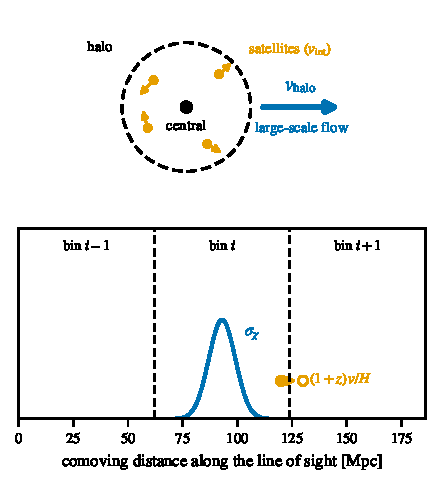
\includegraphics[width=0.72\linewidth]{plots/velocity_schematic/velocity_schematic.pdf}
  \caption{The two parts of a galaxy's velocity
    (Eq.~\eqref{eq:twoparts}), and the blur they produce.  Top: a halo
    drifts as a whole with the large-scale flow ($v_{\rm halo}$,
    Section~\ref{sec:linear}), while its central sits near the center
    and its satellites orbit inside it ($v_{\rm int}$,
    Sections~\ref{sec:virial}--\ref{sec:average}).  Bottom: the
    line-of-sight velocity shifts a galaxy's apparent comoving
    position by $(1 + z)\,v/H(z)$ (Eq.~\eqref{eq:doppler}; filled
    circle the true position, open circle the apparent one), so a
    galaxy near a bin edge is counted in the neighbouring bin and the
    bin's galaxies smear by $\sigma_\chi$; the blur and the
    $62$~Mpc bin width are drawn to scale at $z = 0.5$.}
  \label{fig:schematic}
\end{figure}

\subsection{Step 1: how fast matter moves inside a halo}
\label{sec:virial}

\paragraph{Virial equilibrium, in plain words.}
A halo is a region that has collapsed under its own gravity and settled
into a steady state: its particles orbit in the common potential well,
falling in and swinging out, with no net contraction or expansion.  In
such a state the virial theorem ties the kinetic energy $T$ to the
gravitational potential energy $W$, $2T = -W$ up to boundary terms, so the typical
squared velocity is set by the well's depth:
$\sigma^2 \sim G M / R$, with $M$ the halo's mass and $R$ its radius.
Deeper well, faster orbits.

\paragraph{The radius is not free.}
A halo's ``edge'' is a convention: the radius inside which the mean
density exceeds a chosen threshold $\Delta$ times a reference density.
The common choice $M_{200c}$ uses $\Delta = 200$ times the
\emph{critical} density $\rho_c(z) = 3 H^2(z)/(8\pi G)$:
\begin{equation}
  M_{200c} \;=\; \frac{4\pi}{3}\,200\,\rho_c(z)\,R_{200c}^3
  \;=\; \frac{100\,H^2(z)\,R_{200c}^3}{G} .
  \label{eq:m200c}
\end{equation}
Solving for $R_{200c}$ and inserting it into $\sigma^2 \sim GM/R$
gives the scaling that organizes everything below:
\begin{equation}
  \sigma^2 \;\propto\; G M^{2/3} H^{2/3}(z)
  \qquad\Longrightarrow\qquad
  \shalo \;\propto\; \bigl[M\,H(z)\bigr]^{1/3} .
  \label{eq:scaling}
\end{equation}
The mass enters as $M^{1/3}$: a thousand times more massive halo is
only ten times faster inside.  And at fixed mass a halo at higher
redshift is faster, because the universe was denser, so the same mass
fits inside a smaller, deeper well.

\paragraph{A worked normalization.}
The simplest concrete profile is the singular isothermal sphere, a
halo with a flat circular-velocity curve $V_c^2 = G M(<r)/r$, with
$M(<r)$ the mass enclosed within $r$; a standard property of this
profile is that its
one-dimensional velocity dispersion is $\sigma = V_c/\sqrt{2}$, so
$\sigma^2 = G M_{200c}/(2 R_{200c})$.  For
$M_{200c} = 10^{15}\,\Msun$ at $h(z) \equiv H(z)/(100\kms/{\rm Mpc})
= 1$, Eq.~\eqref{eq:m200c} gives $R_{200c} = 1.63$~Mpc and
$\sigma = 1150\kms$ (with
$G = 4.30 \times 10^{-9}\,{\rm Mpc}\,({\rm km/s})^2/\Msun$, so that
masses in $\Msun$ and lengths in Mpc give velocities in km/s).

\paragraph{The simulation calibration.}
Evrard et al.~\cite{Evrard2008} measured this relation in an ensemble
of N-body simulations.  They define $\shalo$ as the one-dimensional
dispersion of the dark-matter particle velocities, averaged over the
three components,
$\shalo^2 = (3N_p)^{-1}\sum_{i}\sum_{j=1}^{3}|v_{i,j} - \bar{v}_j|^2$,
for halos of mass $M_{200c}$, and fit
\begin{equation}
  \shalo(M, z) \;=\; 1082.9 \pm 4.0\kms\;
  \biggl[\frac{h(z)\, M_{200c}}{10^{15}\,\Msun}\biggr]^{0.3361 \pm 0.0026} ,
  \label{eq:evrard}
\end{equation}
with a log-normal scatter of $4.3\%$ at fixed mass.  Three readings of
Eq.~\eqref{eq:evrard}.  First, the slope is the virial $1/3$ of
Eq.~\eqref{eq:scaling} to one percent, across five decades of mass.
Second, the normalization sits $6\%$ below the isothermal-sphere
estimate above -- the dimensional argument is honest.  Third, the
$h(z)$ factor is exactly the $[M H(z)]^{1/3}$ scaling: with the mass
in $\Msun/h$, as the DESI papers quote it,
$h(z)\,M[\Msun] = E(z)\,M[\Msun/h]$, where $E(z) = H(z)/H_0$.

\begin{figure}[tbp]
  \centering
  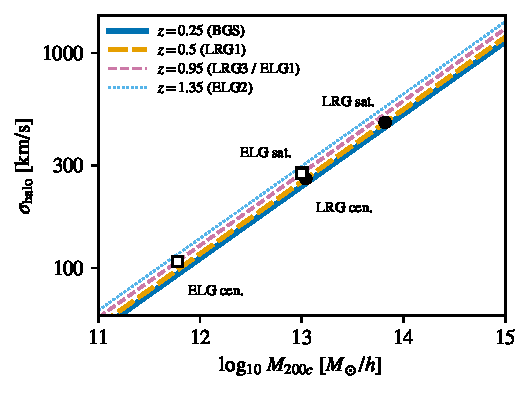
\includegraphics[width=0.72\linewidth]{plots/halo_virial/halo_virial.pdf}
  \caption{The virial velocity $\shalo(M_{200c}, z)$ of
    Eq.~\eqref{eq:evrard} at the mean redshifts of four dispersion
    groups.  Filled circles: the mean host masses of the DESI LRG
    centrals and satellites at $z = 0.5$ (Sections~\ref{sec:hod}
    and~\ref{sec:average}); open squares: the ELG centrals and
    satellites at $z = 0.95$.  The singular-isothermal-sphere estimate
    at $z = 0.5$ is not drawn; it runs $6\%$ above the $z = 0.5$
    curve.}
  \label{fig:virial}
\end{figure}

\paragraph{Worked numbers at the DESI masses.}
Figure~\ref{fig:virial} draws Eq.~\eqref{eq:evrard} at the group
redshifts, with the host masses derived in the next two steps marked.
At $z = 0.5$ ($E = 1.31$): a halo of $10^{13.3}\,\Msun/h$ -- the
two-mass toy's stand-in for the LRG centrals' hosts -- has
$\shalo = 318\kms$, and one of $10^{13.9}\,\Msun/h$ -- the satellites'
hosts -- has $506\kms$.  At the mean host masses of the full
calculation of Section~\ref{sec:average}, $10^{13.04}$ and
$10^{13.82}\,\Msun/h$, the values are $260$ and $476\kms$.  At
$z = 0.95$ the mean ELG host of $10^{11.78}\,\Msun/h$ gives only
$107\kms$: ELGs live in halos about twenty times lighter than the LRG
centrals' hosts and a hundred times lighter than the LRG satellites'
hosts, and that, through $M^{1/3}$, is why their dispersions are the
smallest of the survey.

\paragraph{Mass definitions differ, and it matters at the few-percent
level.}
The DESI fits quote CompaSO halo masses: the total mass of the
particles competitively assigned to the halo~\cite{Rocher2023,
Hadzhiyska2022}, whose outer boundary is a spherical-overdensity
threshold $\Delta_{L1}(z) = (200/18\pi^2)\,\Delta_{\rm BN}(z)$ relative
to critical, with $\Delta_{\rm BN}$ the spherical-collapse fit of
Bryan and Norman~\cite{BryanNorman1998} ($18\pi^2 + 82x - 39x^2$,
$x = \Omega_m(z) - 1$).  At $z = 0.5$ that threshold is $155\,\rho_c$,
looser than Evrard's $200\,\rho_c$, so a CompaSO sphere reaches
further out and holds more mass: for an NFW halo of concentration
$5$--$7$, $M_{L1}/M_{200c} \simeq 1.07$--$1.08$ at $z = 0.5$, falling
to $1.04$ at $z = 0.95$ and $1.03$ at $z = 1.35$ as
$\Delta_{L1} \to 200\,\rho_c$ (an estimate from the profile alone; the
competitive assignment can only remove mass).  Plugging a raw CompaSO
mass into Eq.~\eqref{eq:evrard} therefore overestimates $\shalo$ by
about $(M_{L1}/M_{200c})^{1/3} - 1 \approx 2$--$3\%$ at $z = 0.5$ and
by about $1\%$ at the ELG redshifts.  This note's numbers absorb no
such conversion: a $2$--$3\%$ bias on $\shalo$ is far below the
velocity-bias and satellite-fraction uncertainties of the next steps,
but it belongs on any future precision budget.

\subsection{Step 2: galaxies in halos -- occupation and velocity bias}
\label{sec:hod}

\paragraph{The HOD, in plain words.}
A halo occupation distribution (HOD) gives, for a halo of mass $M$,
the mean number of galaxies of the sample it hosts, split into a
\emph{central} -- at most one, sitting near the halo's center -- and
\emph{satellites}, orbiting inside it.  The LRG fits use the standard
five-parameter form of Zheng et al.~\cite{Zheng2007}, as AbacusHOD
writes it~\cite{Yuan2022}:
\begin{equation}
  \langle N_c\rangle(M) = \tfrac{1}{2}\,{\rm erfc}\!\left[
    \frac{\log_{10}(M_{\rm cut}/M)}{\sqrt{2}\,\sigma}\right] ,
  \qquad
  \langle N_s\rangle(M) = \left[\frac{M - \kappa M_{\rm cut}}
    {M_1}\right]^{\alpha} \langle N_c\rangle(M) .
  \label{eq:zheng}
\end{equation}
Read it as follows: ${\rm erfc}$ is the complementary error function,
falling smoothly from $2$ to $0$, so $\langle N_c\rangle$ turns on
around the mass scale $M_{\rm cut}$ (where it equals $1/2$) over a
width $\sigma$ in dex (decimal exponents: $0.3$~dex is a factor
$10^{0.3} \approx 2$ in mass); satellites appear above $\kappa M_{\rm cut}$
and their number grows as a power law, reaching about one per halo at
$M_1$, typically ten times $M_{\rm cut}$.

\begin{table}[tbp]
  \centering
  \begin{tabular}{lcccc}
    \hline
    & \multicolumn{2}{c}{$\xi(r_p, r_\pi) + n(z)$ fits}
    & \multicolumn{2}{c}{$w_p + n(z)$ fits} \\
    LRG & $0.4 < z < 0.6$ & $0.6 < z < 0.8$
        & $0.8 < z < 0.95$ & $0.95 < z < 1.1$ \\
    \hline
    $\log_{10} M_{\rm cut}$ & $12.79$ & $12.64$ & $12.89$ & $12.68$ \\
    $\log_{10} M_1$ & $13.88$ & $13.71$ & $13.96$ & $13.60$ \\
    $f_{\rm sat}$ & $0.106 \pm 0.012$ & $0.136 \pm 0.011$
                  & $0.110 \pm 0.014$ & $0.151 \pm 0.045$ \\
    $\log_{10}\overline{M}_h$ & $13.40 \pm 0.02$ & $13.24 \pm 0.02$
                  & $13.29 \pm 0.02$ & $13.00 \pm 0.03$ \\
    $\alpha_c$ & $0.33^{+0.05}_{-0.07}$ & $0.19^{+0.06}_{-0.09}$
               & -- & -- \\
    $\alpha_s$ & $0.80 \pm 0.07$ & $0.95^{+0.07}_{-0.06}$ & -- & -- \\
    completeness $f_{\rm ic}$ & $0.70$ & $0.62$
               & $0.92$ & $0.19$ \\
    linear bias $b$ & $1.93$ & $2.08$ & $2.31$ & $2.13$ \\
    \hline
  \end{tabular}
  \caption{The DESI One-Percent LRG HOD fits~\cite{Yuan2023}: the two
    $z < 0.8$ bins fitted to the redshift-space correlation function
    $\xi(r_p, r_\pi)$ ($r_p$, $r_\pi$ the pair separations across and
    along the line of sight), which constrains the velocity biases, and the
    two $z > 0.8$ bins fitted to the projected clustering $w_p$, which
    is blind to velocities.  Masses in $\Msun/h$;
    $\overline{M}_h$ is the mean host mass per galaxy.  The authors
    flag that fixed-redshift snapshots bias the $\overline{M}_h$
    comparison between bins.}
  \label{tab:lrgfits}
\end{table}

\paragraph{The DESI LRG fits.}
Table~\ref{tab:lrgfits} collects what this note needs from the
One-Percent fits~\cite{Yuan2023}.  The satellite fraction
$f_{\rm sat}$ -- the fraction of the sample's galaxies that are
satellites -- rises from $9$--$11\%$ at $z \simeq 0.5$ to $15\%$ in
the last bin ($w_p$ series: $8.9$, $10.4$, $11.0$, $15.1\%$), while
the mean host mass falls from $\log_{10}\overline{M}_h = 13.42$ to
$13.00$ ($w_p$ series).  The last bin is special.  The sample's
completeness $f_{\rm ic}$ (the overall factor by which the fitted
occupation is scaled down, absorbing targets the selection misses)
collapses from $0.92$ to $0.19$, and the linear bias $b$ (the factor
by which the sample's density contrast exceeds the matter's on large
scales) drops from
$2.31$ to $2.13$, all within $\Delta z \approx 0.15$: the selection,
not the halos, changes there.  Section~\ref{sec:literature} builds the
``selection edge'' residual prior on exactly this behavior.

\paragraph{Velocity bias: the definitions.}
Galaxies need not move exactly like the dark matter of their halos,
and the fits parameterize the difference~\cite{Yuan2022}:
\begin{itemize}
  \item \textbf{Centrals.}  The central sits on the halo's central
    subhalo and gets an extra Gaussian line-of-sight velocity,
    $v_{{\rm cen},z} = v_{{\rm halo},z} + \alpha_c\,
    \delta v(\sigma_{\rm LOS})$, where $\delta v$ is a Gaussian draw of
    width equal to the halo's own particle dispersion.  So $\alpha_c$
    is the central's residual dispersion \emph{in units of}
    $\shalo$; $\alpha_c = 0$ means the central rides the halo exactly.
  \item \textbf{Satellites.}  Each satellite rides a halo particle
    with its velocity rescaled about the halo's bulk motion,
    $v_{{\rm sat},z} = v_{{\rm halo},z} + \alpha_s\,
    (v_{{\rm p},z} - v_{{\rm halo},z})$.  So $\alpha_s$ multiplies the
    satellite dispersion relative to $\shalo$; $\alpha_s = 1$ means
    satellites move like the dark matter.
  \item \textbf{ELGs.}  The ELG fits~\cite{Rocher2023} use a different
    but equivalent satellite convention: satellite velocities are
    drawn from a Gaussian about the halo's velocity with width
    $f_{\sigma_v}\,\shalo$, so $f_{\sigma_v}$ plays the role of
    $\alpha_s$.  Their centrals sit at the halo center with the halo's
    velocity: the ELG model has no central velocity bias
    ($\alpha_c \equiv 0$).
\end{itemize}
The fitted values (Table~\ref{tab:lrgfits} and~\cite{Rocher2023}):
for LRGs $\alpha_c = 0.33 \to 0.19$ and $\alpha_s = 0.80 \to 0.95$
between the two $z < 0.8$ bins, and for ELGs
$f_{\sigma_v} = 1.71^{+0.11}_{-0.14}$ at $\bar{z} = 0.95$ and
$1.71^{+0.20}_{-0.15}$ at $1.325$ -- ELG satellites move
\emph{faster} than the dark matter, by $70\%$.  These numbers come
only from the redshift-space fits: the projected clustering $w_p$
integrates the line-of-sight direction away and cannot see
velocities.

\paragraph{The ELG occupation.}
The ELG fits (the mHMQ model~\cite{Rocher2023}: an occupation whose
mean central count peaks near a characteristic mass and falls in
heavier halos, as expected for star-forming galaxies, with
``conformity'' letting satellites prefer halos whose central is itself
an ELG) give
$f_{\rm sat} = 2.6 \pm 0.5\%$ at $\bar{z} = 0.95$ and
$3.5 \pm 1.0\%$ at $1.325$, with mean host mass
$\log_{10}\langle M_h\rangle = 11.78 \to 11.86$ -- every change
within $1\sigma$.  The satellite fraction is model dependent: a
phase-space model fitted to DESI Y1 ELGs finds
$9.5\%$~\cite{Favole2025}, nearly four times larger.
Section~\ref{sec:sum} shows the project's ELG dispersions sit between
the two.

\subsection{Step 3: the galaxy-weighted average}
\label{sec:average}

\paragraph{The mixture rule.}
The sample's internal dispersion $\shod$ averages over two
populations with zero-mean velocities: centrals, dispersion
$\alpha_c\shalo(M_c)$ in their hosts of typical mass $M_c$, and
satellites, $\alpha_s\shalo(M_s)$ in heavier hosts $M_s$.  For a
mixture of zero-mean populations the \emph{variances} add with the
number fractions:
\begin{equation}
  \shod^2 \;=\; (1 - f_{\rm sat})\,\alpha_c^2\,\shalo^2(M_c)
  \;+\; f_{\rm sat}\,\alpha_s^2\,\shalo^2(M_s) .
  \label{eq:mixture}
\end{equation}
Never average the dispersions themselves.  Worked, for the LRG toy at
$z = 0.5$ ($f_{\rm sat} = 0.10$, $\alpha_c = 0.3$, $\alpha_s = 0.9$,
$M_c = 10^{13.3}$, $M_s = 10^{13.9}\,\Msun/h$): centrals contribute
$0.9 \times (0.3 \times 318)^2 = 0.9 \times 95^2$, satellites
$0.1 \times (0.9 \times 506)^2 = 0.1 \times 455^2$, so
$\shod^2 = 8{,}190 + 20{,}730 = (170\kms)^2$.  The wrong,
dispersion-averaged number would be
$0.9 \times 95 + 0.1 \times 455 = 131\kms$, $23\%$ low: the rare, fast
satellites dominate the variance ($72\%$ of it from $10\%$ of the
galaxies), and squaring before averaging is what lets them.

\paragraph{The full mass integral.}
Eq.~\eqref{eq:mixture} compresses an integral over the halo mass
function $n(M)$, the number density of halos per unit mass:
\begin{equation}
  \shod^2 \;=\; \frac{1}{\bar{n}_g}\int\! dM\; n(M)\,
  \Bigl[\langle N_c\rangle(M)\,\alpha_c^2
      + \langle N_s\rangle(M)\,\alpha_s^2\Bigr]\,\shalo^2(M) ,
  \label{eq:integral}
\end{equation}
with $\bar{n}_g = \int dM\, n(M)\,\langle N_c + N_s\rangle$ the
sample's number density.
Evaluating it with the Sheth--Tormen mass
function~\cite{ShethTormen1999} built from the note's fiducial $P(k)$
and the $0.4 < z < 0.6$ LRG fit of Table~\ref{tab:lrgfits} gives
$f_{\rm sat} = 0.116$ (the fit's own $0.106 \pm 0.012$),
mean host masses $\log_{10}M = 13.04$ for centrals and $13.82$ for
satellites, and $\shod = 171\kms$ -- the two-mass toy's $170\kms$ to
better than one percent.  The toy is quantitatively trustworthy
because each population's $\shalo^2$ is dominated by a narrow range of
host masses.  The same integral at the $0.6 < z < 0.8$ fit gives
$\shod = 188\kms$ (these are estimates built on the quoted fits, not
published numbers).

\begin{figure}[tbp]
  \centering
  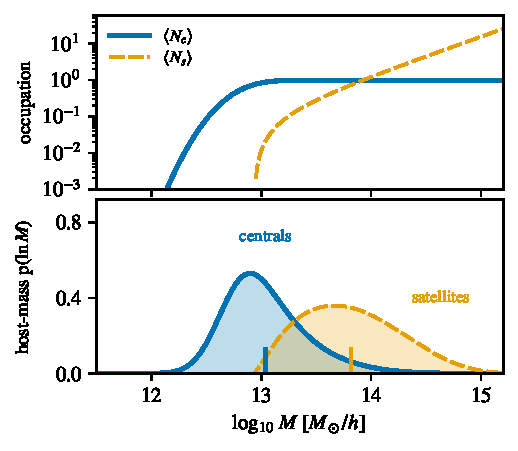
\includegraphics[width=0.72\linewidth]{plots/hod_weights/hod_weights.pdf}
  \caption{The LRG occupation at $z = 0.5$
    (Eq.~\eqref{eq:zheng} with the $0.4 < z < 0.6$ fit of
    Table~\ref{tab:lrgfits}) and the host-mass distributions
    $p(\ln M) \propto n(M)\,M\,\langle N\rangle$ of its centrals and
    satellites on a Sheth--Tormen mass function at the note's
    fiducial cosmology, each normalized to unit area; vertical ticks
    mark the mean host masses.  Satellites occupy halos about six
    times heavier than centrals.}
  \label{fig:hodweights}
\end{figure}

\paragraph{Why satellites sit in heavier halos.}
Figure~\ref{fig:hodweights} shows the two host-mass distributions.
Centrals pile up just above $M_{\rm cut}$, where halos are still
abundant; satellites need $\langle N_s\rangle$ to be appreciable,
which happens only towards $M_1 \approx 10\,M_{\rm cut}$, and massive
halos host many of them at once.  The mean satellite host,
$10^{13.8}\,\Msun/h$, is six times the mean central host -- hence
nearly twice the virial velocity, and, squared, the dominance in
Eq.~\eqref{eq:mixture}.

\paragraph{A subtlety: which average enters the two-halo damping.}
Eq.~\eqref{eq:integral} weights each galaxy equally.  In halo-model
redshift space the damping of the \emph{two-halo} (large-scale) power
enters differently: each galaxy's Fingers-of-God kernel is carried
inside the galaxy-bias integral, weighted by its halo's clustering
bias $b(M)$, the mass-dependent version of the sample bias $b$ above,
rising with mass~\cite{White2001, Seljak2001}, and in the low-$k$
expansion the leading damping term is
$\propto \int dM\, n(M)\, b(M)\, \langle N_s\rangle\, \sigma_u^2(M)$,
with $\sigma_u(M)$ the halo's internal dispersion expressed as a
comoving displacement, $(1+z)\,\shalo(M)/H(z)$ as in
Eq.~\eqref{eq:doppler}~\cite{Maus2024}.  Two consequences.  Heavier halos, with larger
$b(M)$, count more, so the effective two-halo dispersion is somewhat
larger than the galaxy-weighted one.  And in these models only the
satellite term is damped -- a central sits at its halo's center and
carries no internal displacement -- while the measured
$\alpha_c > 0$ adds a small central damping on top.  The project's
blur applies one galaxy-weighted $\sv$ to the whole bin; the
difference between the weightings is a modest, mass-function-weighted
systematic that the $\sv$ priors must cover, not a separate parameter.

\subsection{Step 4: the halos' own motion -- the linear flow}
\label{sec:linear}

\paragraph{From the growth of structure to a velocity.}
On large scales matter conserves mass while it clusters, so the
density contrast $\delta$ and the peculiar velocity field ${\bf v}$
obey the linearized continuity equation
$\dot{\delta} = -\nabla\!\cdot\!{\bf v}/a$, with $a = 1/(1+z)$ the
scale factor and the gradient in comoving coordinates.  In linear
theory every Fourier mode grows with the same factor $D(z)$ (the
linear growth factor, $D(0) = 1$), so
$\dot{\delta} = \delta\, \dot{D}/D = \delta\, H f$ with
$f \equiv d\ln D/d\ln a$ the growth rate (the chain rule:
$\dot{D}/D = H\, d\ln D/d\ln a$).  In Fourier space the divergence
becomes $i{\bf k}\cdot{\bf v}_{\bf k}$, and a linear flow is
irrotational (any initial rotation decays with the expansion), so
${\bf v}_{\bf k}$ points along ${\bf k}$.  Solving the continuity
equation for the velocity of mode ${\bf k}$,
\begin{equation}
  {\bf v}_{\bf k} \;=\; i\, a H f\, \delta_{\bf k}\,
  \frac{{\bf k}}{k^2}
  \qquad\Longleftrightarrow\qquad
  {\bf v} \;=\; a H f\, \boldsymbol{\Psi} ,
  \label{eq:vlin}
\end{equation}
where $\boldsymbol{\Psi}$ is the linear displacement field, the vector
whose divergence is $-\delta$.  A patch of matter moves with velocity
$aHf$ times the displacement that built its environment.

\paragraph{The one-point dispersion.}
The power spectrum measures the variance of the modes:
$\langle\delta_{\bf k}\delta^*_{{\bf k}'}\rangle =
(2\pi)^3\delta_D({\bf k} - {\bf k}')\,P_{\rm lin}(k)$, with $\delta_D$
the Dirac delta.  Each mode of Eq.~\eqref{eq:vlin} then contributes
$(aHf)^2 P_{\rm lin}(k)/k^2$ to the velocity variance, and summing the
modes, $\int\! d^3k\,(2\pi)^{-3}\, P_{\rm lin}(k)/k^2 =
(2\pi^2)^{-1}\!\int\! P_{\rm lin}(k)\,dk$, gives the three-dimensional
variance $(aHf)^2 (2\pi^2)^{-1}\!\int\! P_{\rm lin}(k)\,dk$; one
line-of-sight component carries a third of it:
\begin{equation}
  \slin(z) \;=\; \frac{H(z)}{1+z}\, f(z)\, \sigma_d(z) ,
  \qquad
  \sigma_d^2(z) \;=\; \frac{1}{6\pi^2}\int_0^\infty
  P_{\rm lin}(k, z)\, dk \;=\; D^2(z)\,\sigma_{d,0}^2 .
  \label{eq:siglin}
\end{equation}
$\sigma_d$ is the one-dimensional rms linear displacement.  The
integral converges at both ends ($P \propto k$ at low $k$,
$\propto k^{n_s - 3}\ln^2 k$ at high $k$) and is dominated by
$k \sim 0.01$--$0.3\hMpc$; at the fiducial cosmology
$\sigma_{d,0} = 8.86$~Mpc $= 5.96\Mpch$, stable to $0.03\%$ between
upper cutoffs of $10$ and $80/{\rm Mpc}$.

\paragraph{Worked values, and why the curve is so flat.}
At the group redshifts $\bar{z}_g = 0.18$, $0.33$, $0.50$, $0.70$,
$0.95$, $1.35$ the fiducial gives $\slin = 309$, $307$, $301$, $293$,
$282$, $263\kms$.  Three factors nearly cancel: $D(z)$ falls, $f(z)$
rises towards $1$ (matter domination), and $H(z)/(1+z)$ passes
through a shallow minimum.  The net logarithmic slope
$d\ln\slin/dz$ is $-0.01$ at $z = 0.18$, $-0.12$ at $0.5$ and
$-0.17$ at $1.35$.  Cosmology fixes this part, it is smooth in
redshift, and the Fisher forecasts hold it at the fiducial (the blur
carries no cosmological information by construction) -- so
\emph{per-bin scatter can live only in the halo part}.

\paragraph{Halos move slightly differently from the matter.}
$\slin$ is the dispersion of a random patch of matter.  Halos are not
random patches: they form at peaks of the initial field, and a peak's
velocity is pulled down by the correlation between its height and the
surrounding flow.  For Gaussian initial conditions the reduction is
the peak-constraint factor $[1 - \sigma_0^4/(\sigma_1^2
\sigma_{-1}^2)]^{1/2}$ evaluated with the field smoothed on the halo's
Lagrangian scale -- the comoving radius of the sphere that held the
halo's mass before collapse, $R = [3M/(4\pi\bar{\rho}_m)]^{1/3}$, a
few Mpc here~\cite{BBKS1986, ShethDiaferio2001}.  Here
$\sigma_j^2 = (2\pi^2)^{-1}\!\int\!dk\,k^{2+2j}P(k)W^2(kR)$ are
smoothed spectral moments: weighted variances of the field, $j = 0$
the density itself, negative $j$ weighing large scales more, with
$W(kR)$ the Fourier transform of the smoothing sphere.  At the fiducial $P(k)$ the factor is
$0.98$ at the mean ELG host mass, $0.95$ at $10^{13.4}$ and $0.93$ at
$10^{13.9}\,\Msun/h$: a few-percent slowdown, growing with mass.
Working against it, halo speeds grow \emph{faster} than linear theory
in dense regions, by tens of percent for massive halos with massive
neighbours~\cite{ShethDiaferio2001}.  The two corrections pull in
opposite directions and neither is computed for the DESI samples, so
this note treats the halo-motion part as $\slin$ with a
several-percent uncertainty; Section~\ref{sec:model} charges it to
the halo share $w$ as $\pm 0.05$.

\subsection{Adding the two parts: $\sv^2 = \slin^2 + \shod^2$}
\label{sec:sum}

\paragraph{Why the variances add.}
The two parts of Eq.~\eqref{eq:twoparts} are uncorrelated at leading
order: whether a satellite is currently moving towards us or away on
its orbit does not depend on which way its halo drifts, so
$\langle v_{\rm halo}\, v_{\rm int}\rangle = 0$ and
\begin{equation}
  \sv^2 \;=\; \slin^2 \;+\; \shod^2 .
  \label{eq:sum}
\end{equation}
The argument has limits.  Both parts respond to the same environment
(halos in dense regions are both faster and more satellite rich), the
halo-motion part carries the quasilinear corrections of
Section~\ref{sec:linear}, and a simulation's measured one-point
dispersion contains everything at once.  So when this note
``inverts'' Eq.~\eqref{eq:sum} below, the inferred $\shod$ is really
\emph{everything the linear flow does not explain}, internal motions
plus nonlinear flow corrections.  With that reading, worked at the
toy: $\sqrt{300^2 + 170^2} = 345\kms$, squarely inside the LRG
fiducials $343$--$357\kms$.  The chain from the virial theorem to the
measured dispersions closes.

\begin{table}[tbp]
  \centering
  \begin{tabular}{lccccc}
    \hline
    group & $\bar{z}_g$ & $\sv$ & $\slin(\bar{z}_g)$
    & $\shod(\bar{z}_g)$ & $w = \shod^2/\sv^2$ \\
    \hline
    BGS0 & $0.18$ & $371$ & $309$ & $206$ & $0.31$ \\
    BGS1 & $0.33$ & $358$ & $307$ & $185$ & $0.27$ \\
    LRG1 & $0.50$ & $357$ & $301$ & $191$ & $0.29$ \\
    LRG2 & $0.70$ & $348$ & $293$ & $187$ & $0.29$ \\
    LRG3 & $0.95$ & $343$ & $282$ & $196$ & $0.33$ \\
    ELG1 & $0.95$ & $304$ & $282$ & $114$ & $0.14$ \\
    ELG2 & $1.35$ & $289$ & $263$ & $119$ & $0.17$ \\
    \hline
  \end{tabular}
  \caption{The decomposition of each group's fiducial dispersion at
    its mean redshift (all velocities in km/s): the linear flow from
    the fiducial CAMB $P(k)$ (Eq.~\eqref{eq:siglin}), the halo part by
    subtraction ($\shod^2 = \sv^2 - \slin^2$), and the halo share $w$
    of the variance.  $\bar{z}_g$ of the $\Delta z = 0.02$ layout.}
  \label{tab:decomposition}
\end{table}

\paragraph{The decomposition per group.}
Table~\ref{tab:decomposition} inverts Eq.~\eqref{eq:sum} at each
group's mean redshift, and Figure~\ref{fig:decomposition} does it bin
by bin on $\Delta z = 0.02$.  The halo share of the variance is
$w = 0.27$--$0.33$ for BGS and LRG and $0.14$--$0.17$ for ELG.  These
shares control everything in Section~\ref{sec:model}: a fractional
change $\delta\shod/\shod$ moves $\sv$ by only
$w\,\delta\shod/\shod$, so a $10\%$ halo-part wiggle is a $3\%$
dispersion wiggle for LRGs and $1.5\%$ for ELGs.

\begin{figure}[tbp]
  \centering
  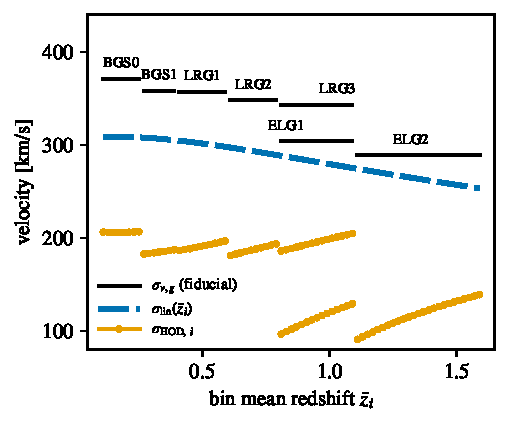
\includegraphics[width=0.78\linewidth]{plots/lin_decomposition/lin_decomposition.pdf}
  \caption{The decomposition per bin on $\Delta z = 0.02$: the
    fiducial $\svg$ (flat per group), the linear flow
    $\slin(\bar{z}_i)$, and the implied halo part
    $\shod{}_{,i} = (\svg^2 - \slin^2(\bar{z}_i))^{1/2}$.  Where two
    groups share a redshift range (LRG3 and ELG1), the ELG group is
    the lower pair of lines.  The rise of $\shod{}_{,i}$ inside each
    group is the $T_{\rm lin}$ truth of Section~\ref{sec:study}: a
    flat $\sv$ forces the halo part to climb against the falling
    linear flow.}
  \label{fig:decomposition}
\end{figure}

\paragraph{Three consistency checks.}
First, LRG1: the halo model predicts $\shod = 171\kms$
(Section~\ref{sec:average}); the subtraction gives $191\kms$ -- a
$10\%$ agreement with no tuning, well inside the velocity-bias error
bars and the halo-motion uncertainty.  Second, LRG2: the full
integral at the $0.6 < z < 0.8$ fit predicts $188\kms$ against the
subtracted $187\kms$ (the exactness is luck; both fits carry
$\sim 10\%$ uncertainties).  Third, ELG: the subtraction gives
$114$--$119\kms$, while the halo model gives $76\kms$ with the
One-Percent occupation ($f_{\rm sat} = 0.026$,
$f_{\sigma_v}\shalo$ at the satellite hosts near
$10^{13}\,\Msun/h$) and $145\kms$ with the $9.5\%$ satellite fraction
of~\cite{Favole2025} (both estimates).  The project's ELG dispersions
sit between the two published occupations: the ELG halo part is real
but model dependent at the factor-two level, which is a reason to
keep its per-bin freedom fractional in $\shod$ rather than absolute.

\paragraph{What the halo model then predicts for redshift trends.}
Between the two LRG $\xi$ fits the full integral's $\shod$ rises from
$171$ to $188\kms$ over $\Delta z = 0.2$: a slope
$d\ln\shod/dz \approx +0.5$ per unit $z$ (estimate).  The two-mass
toy decomposes the competing effects: the host-mass decline
($\log_{10}\overline{M}_h$ $13.42 \to 13.00$ across
$\bar{z} = 0.5 \to 1.03$) with $\shalo \propto (M E(z))^{1/3}$ gives
$d\ln\shalo/dz \approx -0.41$, while the rising satellite fraction
($8.9 \to 15.1\%$, $w_p$ series) gives about $+0.4$, and the fitted
velocity-bias changes ($\alpha_s$ up, $\alpha_c$ down) partly cancel
each other ($+13\%$ and $-11\%$ on $\shod$).  The honest conclusion:
the sign of the LRG slope is not established, and magnitudes up to
$|d\ln\shod/dz| \sim 0.5$ are easy to produce.  That is the slope
prior's scale.

\subsection{One-point versus pairwise dispersions}
\label{sec:pairwise}

\paragraph{Two different statistics.}
The blur needs the \emph{one-point} dispersion: the rms velocity of
single galaxies.  Most measurements quote a \emph{pairwise}
dispersion $\sigma_{12}(r)$: the rms of the velocity difference
between two galaxies separated by $r$.  For zero-mean line-of-sight
velocities with one-point variance $\sigma_{\rm 1pt}^2$ and two-point
correlation $\psi(r) = \langle v_1 v_2\rangle$,
\begin{equation}
  \sigma_{12}^2(r) \;=\;
  \bigl\langle (v_1 - v_2)^2 \bigr\rangle
  \;=\; 2\,\bigl[\sigma_{\rm 1pt}^2 - \psi(r)\bigr] .
  \label{eq:pairwise}
\end{equation}
At small separations the coherent flow moves both members of a pair
together, so its contribution cancels ($\psi \to$ the flow's
variance) and what survives is twice the \emph{internal} variance of
the pair's halo; at large separations $\psi \to 0$ and
$\sigma_{12} \to \sqrt{2}\,\sigma_{\rm 1pt}$.  On top of that, pairs
are counted per pair, $\propto N(N-1)$, so a halo with $N$ satellites
contributes $N(N-1)/2$ one-halo pairs: rich clusters dominate
pairwise statistics far more than they dominate the galaxy count.

\paragraph{What the classic numbers actually are.}
In CfA2+SSRS2, $\sigma_{12} = 540 \pm 180\kms$ at
$r \sim 1\Mpch$~\cite{Marzke1995}; removing the Abell $R \ge 1$
clusters drops it to $295 \pm 99\kms$, and the subvolume-to-subvolume
scatter is dominated by whether a rich cluster fell in the volume.
In GAMA the small-scale pairwise dispersion rises from about
$200\kms$ at $M_r = -17$ to about $600\kms$ at
$M_r \approx -22$~\cite{Loveday2018}, while HOD models predict the
opposite luminosity trend at small and large $r$, driven by the
falling satellite fraction above $L_*$~\cite{Tinker2007}.  The BOSS
full-shape fits give damping parameters
$\sigma_v = 6.10 \pm 0.69$, $5.84^{+0.70}_{-0.77}$ and
$5.35^{+0.76}_{-0.81}\Mpch$ (NGC) at $z_{\rm eff} = 0.38$, $0.51$,
$0.61$~\cite{Beutler2017}, and VIPERS gives
$\sigma_{12} = 5.00 \pm 0.86$ and $3.54 \pm 0.78\Mpch$ at
$z = 0.6$ and $0.86$~\cite{Pezzotta2017}; converted with
Eq.~\eqref{eq:doppler} at the note's fiducial these are $539$, $509$,
$464\kms$ and $434$, $309\kms$ (estimates).  All of these are
\emph{model} parameters of pairwise-velocity damping templates, fitted
alongside bias and shot noise (the Poisson noise of counting a finite
number of galaxies), not direct one-point measurements.

\paragraph{Why none of them is $\sv$.}
Compare $540\kms$ (CfA2, pair weighted, cluster dominated) with the
project's $371$--$289\kms$ (one point, galaxy weighted): the factor
$\sqrt{2}$ of Eq.~\eqref{eq:pairwise}, the $N(N-1)$ weighting towards
rich halos, and the model dependence each move the number by tens of
percent.  The literature can therefore \emph{bracket} redshift trends
and scatter (Section~\ref{sec:literature}) but cannot replace the
source forecast's own one-point measurement -- which is why the priors
of Section~\ref{sec:model} stay anchored to it.

\subsection{Caveats: the blur's shape, the Kaiser boundary, and
SN$_2$}
\label{sec:caveats}

\paragraph{A mixture is not a Gaussian.}
The blur convolves $n_i(z)$ with one Gaussian of width
$\sigma_{z,i}$.  But Section~\ref{sec:average} built the velocity
distribution as a mass-weighted mixture of Gaussians of very
different widths ($95\kms$ centrals, $455\kms$ satellites), and a
mixture has heavier tails than one Gaussian of the same total
variance -- summed over the halo mass function the tails are close to
exponential~\cite{ShethDiaferio2001}.  The project blurs with one
Gaussian at the mixture's total variance.  How much the tail shape
matters for band powers is an open robustness check (the
Fingers-of-God profile item in the appendix), not settled here.

\paragraph{Possible double counting with the Kaiser term.}
The one-point $\sv$ contains the full linear flow,
$\slin^2 = \sv^2 - \shod^2$ by construction.  The coherent part of
that same flow is what the Kaiser term models as a systematic
distortion of the clustering amplitude.  Blurring the window with the
\emph{full} $\sv$ treats the whole velocity as random scatter
uncorrelated with the density, so the correlated large-scale part
enters twice: once coherently (Kaiser), once as damping (the blur).
Eq.~\eqref{eq:pairwise} shows the size of the ambiguity: a damping
built from pair separations would subtract $\psi(r)$, which at small
$r$ removes most of $\slin^2$ -- precisely the difference between
damping with $\sv^2$ and with $\shod^2$.  The project follows the
source forecast and uses the full measured dispersion; the sixfold
prior widths, introduced for the $\alpha_2$ degeneracy, also cover
this modeling ambiguity.  This note states the issue and does not
settle it; the study's design (per-bin scatter on the halo part only)
is unaffected, because both conventions share the halo part.

\paragraph{The SN$_2$ stochastic term carries the same satellite
velocities.}
The project's one-loop bias model (its perturbation-theory model of
the galaxy power spectrum, \texttt{notes/higher\us order\us bias})
carries a line-of-sight stochastic term
${\rm SN}_2\,k^2\mu^2$, with $\mu$ the cosine of the angle between
${\bf k}$ and the line of sight, in units of
$f_{\rm sat}\sigma_{\rm sat}^2/\bar{n}_i$, the DESI DR1 scaling of
Maus et al.~\cite{Maus2024}: in their halo-model expansion the
one-halo (central--satellite and satellite--satellite) power at low
$k$ contributes a $k^2\mu^2$ white term (white: a constant amplitude
in $k$, like shot noise) of amplitude
$f_{\rm sat}\,\sigma_{1,\rm eff}^2/\bar{n}_g$, with
$\sigma_{1,\rm eff}$ the $\langle N_c N_s\rangle$-weighted satellite
dispersion in distance units.  The code's unit is their
stochastic-prior table: LRG $(f_{\rm sat}, \sigma) = (0.1,
7.8\Mpch)$, ELG $(0.1, 2.9\Mpch)$, BGS borrowing the LRG row
(\texttt{SN2\us UNIT} in \texttt{likelihood/desi\us cl.py}; $6.084$
and $0.841$ $({\rm Mpc}/h)^2$).  Converted with
Eq.~\eqref{eq:doppler}, $7.8\Mpch$ is $677$--$684\kms$ across the LRG
groups -- about $1.5$ times the halo-model satellite dispersion
$\alpha_s\shalo(M_s) \approx 430$--$455\kms \approx 5\Mpch$
(Section~\ref{sec:average}; estimates), so Maus et al.'s number is a
generous order-of-magnitude width, not a measurement.  The ELG unit
assumes $f_{\rm sat} = 0.1$, four times the One-Percent fit.  The
physical point: the blur (window side) and SN$_2$ (one-halo
stochastic side) describe the same satellite virial motions in two
places the projection treats differently; like the $\alpha_2$
degeneracy of the Fingers-of-God note, this is a family of partially
redundant descriptions, and the priors, not a fit, set how the
redundancy is shared.

\section{What the literature says about slopes, scatter and
correlation lengths}
\label{sec:literature}

No published analysis measures the Fingers-of-God dispersion in thin
redshift slices for any DESI tracer.  What exists is HOD fits in
broad bins ($\Delta z = 0.2$--$0.5$), damping fits in broad bins, and
this note's own propagation of them.  The evidence for each number
below is graded explicitly.

\paragraph{Slopes within a sample.}
The linear part falls at $d\ln\slin/dz = -0.01$ to $-0.17$ per unit
$z$ (fiducial $P(k)$, firm).  For the halo part:
the LRG HOD changes between broad bins give slopes of either sign up
to $|d\ln\shod/dz| \approx 0.5$ (Section~\ref{sec:sum}; estimate).
The BOSS damping values above fall as
$d\ln\sigma/dz \approx -1.0 \pm 0.6$ per unit $z$ (a straight-line
fit to the NGC and SGC values; estimate, $1$--$1.5\sigma$,
model-dependent damping of a mixed LOWZ+CMASS sample), and VIPERS
gives $-1.3 \pm 1.0$ (same caveats).  In $\sv$ units every halo-part
slope is multiplied by $w$.  For a flux-limited BGS (a sample limited by apparent brightness, so at
higher redshift only intrinsically brighter galaxies make the cut and
the population itself drifts) the \emph{sign}
is open: the luminosity limit brightens by about $2.5$~mag across
$0.1 < z < 0.4$ (estimate), GAMA's pairwise dispersion rises with
luminosity while HOD models predict it falls~\cite{Loveday2018,
Tinker2007}, and the project already treats BGS as flux limited (its
bias drift in \texttt{scripts/make\us desi\us params.py} comes from
the flux limit).

\paragraph{Where departures cluster: selection edges.}
The sharpest documented population changes sit where the target
selection changes, within $\Delta z \approx 0.1$--$0.15$: the DESI
LRG completeness collapse at $z > 0.95$ (Table~\ref{tab:lrgfits});
and BOSS in thin shells, where no smooth $b(z)$ model fits above
$z \approx 0.6$, the onset of flux-limited behavior, forcing that
analysis to drop its last three shells~\cite{SalazarAlbornoz2017}.
So population departures correlate over $\Delta z \sim 0.1$--$0.3$
inside a group and over $0.05$--$0.1$ near sample edges.  No paper
measures a correlation length for a dispersion; $L$ is argued from
the redshift scale of selection changes, not measured.

\paragraph{A white (uncorrelated) part.}
A finite slice holds a finite number of rich halos, and
Section~\ref{sec:pairwise} showed how strongly they weight velocity
statistics: in CfA2+SSRS2 the spread between subvolumes of about
$7 \times 10^5\,({\rm Mpc}/h)^3$ was cluster
dominated~\cite{Marzke1995}.  Scaling that spread as
$V^{-1/2}$ to a $62$~Mpc slice of the DESI footprint (about
$10^8\,({\rm Mpc}/h)^3$) leaves $\lesssim 3\%$ on the pair-weighted
statistic, and less on the galaxy-weighted $\sv$, which rich halos
dominate more weakly: $\lesssim 1$--$2\%$ of $\shod$ per bin, with
$L$ of about one bin (crude estimate).

\paragraph{Thin-bin precedents.}
The BOSS tomographic analysis closest in spirit to this
project~\cite{SalazarAlbornoz2017} used $18$ thin shells with
\emph{one} Fingers-of-God parameter $a_{\rm vir}$ scaled
deterministically as $(D(z)/D(z_{\rm ref}))^2$ and one linear bias
law $b_1 + b'(z - z_{\rm ref})$: no parameter was free per shell.
For the harmonic-space power spectrum, the Fingers of God suppress
$C_\ell$ on \emph{all} transverse scales once the bin is thinner than
$\Delta r \lesssim \pi\sigma_u$, with $\sigma_u$ the dispersion in
distance units~\cite{GrasshornGebhardt2020} -- for
$\sv = 350\kms$ at $z = 0.5$, $\pi\sigma_u \approx 19$~Mpc, below the
$62$~Mpc bins but not by orders of magnitude; and for
$\Delta z \lesssim 0.01$ nonlinear redshift-space corrections enter
at all $\ell$~\cite{Jalilvand2020}.  No published exponential-kernel
or Gaussian-process prior on a Fingers-of-God parameter across thin
bins was found: the construction below appears to be new in this
context.

\section{The per-bin model}
\label{sec:model}

\paragraph{Where the freedom lives.}
Write each bin's dispersion as Eq.~\eqref{eq:sum} with the linear
part held at the fiducial cosmology.  The fiducial stays exactly
today's: $\sv{}_{,i} = \svg$, flat in each group, so every existing
derivative base remains valid; the implied fiducial halo part
$\shod^2{}_{,i} = \svg^2 - \slin^2(\bar{z}_i)$ rises slightly across
each group (Figure~\ref{fig:decomposition}).  The group \emph{level}
keeps today's parameter and prior (the paper widths of
Table~\ref{tab:sigv}).  The new freedom acts on the halo part only:
\begin{equation}
  \shod{}_{,i} \;\longrightarrow\; \shod{}_{,i}\,
  \bigl[\,1 + s_g\,(\bar{z}_i - \bar{z}_g) + \varepsilon_i\,\bigr] ,
  \label{eq:perbin}
\end{equation}
with $s_g$ a free slope per group and $\varepsilon_i$ a correlated
per-bin residual.

\paragraph{The residual prior, borrowed from the linear bias.}
$\varepsilon$ has the exponential-kernel prior
$\langle\varepsilon_i\varepsilon_j\rangle = \sigma^2
e^{-|\bar{z}_i - \bar{z}_j|/L}$ within a group (zero across groups;
$L$ a correlation length in redshift: residuals of bins closer than
$L$ move together),
\emph{projected} so that it charges (penalizes in the $\chi^2$)
neither the group's level nor its
slope: the prior precision is
$P = Q - QU(U^{\mathsf T}QU)^{-1}U^{\mathsf T}Q$ with $Q$ the inverse
kernel and $U = [1,\, z - \bar{z}_g]$, the construction built and
derived step by step for the linear bias $b_1$ in the correlated-prior
note, \texttt{notes/correlated\us bias\us prior\us v2} (its appendix
sections on the projected precision and the memory projection).  The
level and the slope stay free (the level under today's Gaussian
prior); the kernel constrains only the wiggles around each group's
line.

\paragraph{The linear response, and why no new physics is needed.}
Differentiating $\sv{}_{,i}^2 = \slin^2{}_{,i} + \shod^2{}_{,i}$ at
fixed $\slin$,
$\delta\sv{}_{,i} = (\shod{}_{,i}^2/\sv{}_{,i})\,
(\delta\shod{}_{,i}/\shod{}_{,i})$, so a fractional halo-part change
reaches the sampled dispersion suppressed by the halo share:
\begin{equation}
  \delta\sv{}_{,i} \;=\; w_i\,\svg\,
  \bigl[\,s_g\,(\bar{z}_i - \bar{z}_g) + \varepsilon_i\,\bigr] ,
  \qquad
  w_i = \frac{\shod^2{}_{,i}}{\svg^2} .
  \label{eq:response}
\end{equation}
Every variant of the study is therefore a linear combination of
per-bin $\sv$ derivative columns (a derivative column is the
derivative of the whole data vector with respect to one parameter, the
building block of the Fisher matrix; the machinery note builds
everything from them) -- the slope and residual directions
are those columns weighted by $w_i\svg$ -- and the likelihood needs
no new option: the freedom costs only the per-bin columns
(Section~\ref{sec:study}).  Worked sizes from
Table~\ref{tab:decomposition}: a one-sigma baseline slope
($s_g = 1$ per unit $z$) tilts LRG3's dispersions by
$w\,\Delta z \approx 0.33 \times (\pm 0.14) \approx \pm 4.6\%$ of
$\svg$, about $\pm 16\kms$ across the group; the same slope moves
ELG1 by only $\pm 1.9\%$, the halo share being half as large.

\begin{table}[tbp]
  \centering
  \begin{tabular}{llp{4.5cm}}
    \hline
    piece & prior & where the number comes from \\
    \hline
    level & today's Gaussian, paper widths & Table~\ref{tab:sigv} \\
    slope $s_g$ & $N(0, 0.5/1.0/2.0)$ per unit $z$; BGS $2.0$
      & Section~\ref{sec:sum}; BGS sign open \\
    residual A & $\sigma = 10\%$ of $\shod$, $L = 0.2$
      & broad-bin HOD changes ($7$--$21\%$) \\
    residual B & $\sigma = 20\%$ ($30\%$ BGS), $L = 0.05$
      & selection edges (LRG $z > 0.95$; BOSS $z > 0.6$) \\
    white term (optional) & $5\%$ of $\shod$, $L = 0.02$
      & rich-halo shot noise (crude) \\
    \hline
  \end{tabular}
  \caption{The per-bin priors on the halo part and their provenance.
    In $\sv$ units each width is multiplied by the halo share
    ($w \approx 0.27$--$0.33$ BGS/LRG, $0.14$--$0.17$ ELG): residual
    A is a $3\%$ dispersion wiggle for LRGs and $1.4$--$1.7\%$ for
    ELGs.}
  \label{tab:priors}
\end{table}

\paragraph{How each prior number follows from the physics.}
Table~\ref{tab:priors} summarizes; the trail:
\begin{itemize}
  \item \textbf{Slope widths $0.5/1.0/2.0$.}  Section~\ref{sec:sum}
    produced halo-part slopes of either sign up to
    $|d\ln\shod/dz| \approx 0.5$ from fitted HOD evolution alone;
    $0.5$ is therefore optimistic (the halo model taken at face
    value), $1.0$ baseline (covering the BOSS and VIPERS damping
    trends at about $1\sigma$ once multiplied by $w$), $2.0$
    pessimistic.  BGS takes $2.0$ because its flux-limited slope has
    an open sign (Section~\ref{sec:literature}).
  \item \textbf{Residual A ($10\%$, $L = 0.2$): population drift.}
    The HOD changes the DESI fits find between broad bins move
    $\shod$ by $+7\%$ ($f_{\rm sat}$ $9\% \to 11\%$), $+13\%$
    ($\alpha_s$ $0.80 \to 0.95$), $-11\%$ ($\alpha_c$
    $0.33 \to 0.19$) and $+21\%$ ($f_{\rm sat}$ $8.9 \to 15.1\%$)
    in the two-mass toy; $10\%$ with $L = 0.2$ lets such drifts
    happen on the $\Delta z \sim 0.2$--$0.4$ scale they are observed
    on.
  \item \textbf{Residual B ($20\%$, BGS $30\%$, $L = 0.05$):
    selection edges.}  Population changes concentrate where the
    selection changes within $\Delta z \approx 0.15$
    (Section~\ref{sec:literature}); $20\%$ of $\shod$ is the size of
    the LRG $z > 0.95$ upheaval, and $30\%$ for BGS reflects the
    open sign and the stronger selection drift of a flux-limited
    sample.
  \item \textbf{White term ($5\%$, $L = 0.02$).}  The rich-halo shot
    noise estimate of Section~\ref{sec:literature}, roughly one bin
    in correlation length.  It is a crude number and the term is
    optional.
\end{itemize}

\begin{figure}[tbp]
  \centering
  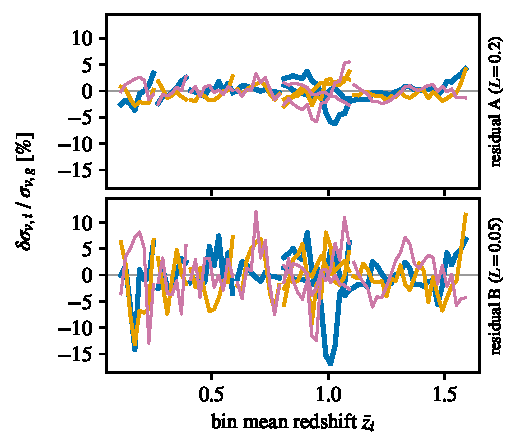
\includegraphics[width=0.78\linewidth]{plots/prior_draws/prior_draws.pdf}
  \caption{Random truths of the per-bin model on $\Delta z = 0.02$,
    as percent of each group's $\svg$
    (Eq.~\eqref{eq:response}; baseline slope width, kernel-projected
    residuals): three draws under residual A (top) and residual B
    (bottom), the same slope draws in both panels, so only the
    residual changes between them.  The largest excursions sit where
    the halo share $w$ is largest (BGS and LRG3); the ELG groups,
    with $w \approx 0.15$, barely move under A.}
  \label{fig:draws}
\end{figure}

\paragraph{What the draws look like.}
Figure~\ref{fig:draws} shows random truths under slope $+$ A and
slope $+$ B.  A produces slow, few-percent breathing of a group's
dispersions; B produces bin-to-bin structure reaching $\pm 10\%$ of
$\sv$ in the high-$w$ groups.  For comparison, the per-bin error bars
of the source forecast's measurement are $2$--$4\%$ of $\sv$ for LRG
and ELG and $6$--$8\%$ for BGS: residual A is at the measurement's
own resolution, residual B deliberately above it.

\paragraph{Robustness of $w$.}
The halo shares inherit the halo-motion uncertainty of
Section~\ref{sec:linear} (peaks slower by $2$--$7\%$, nonlinear
evolution faster by a similar amount, with opposite signs), so $w$
per group is uncertain by roughly $\pm 0.05$.  Since
Eq.~\eqref{eq:response} uses $w_i$ only as a fixed weight on the
derivative columns, a change of $w$ touches no evaluation, only the
weights; the appendix records why no separate refit is needed.

\section{The study}
\label{sec:study}

\paragraph{The accuracy test comes before any FoM.}
A figure of merit from a model that cannot absorb the true signal is
meaningless, so the project always tests accuracy first (the
linear-bias ladder of \texttt{notes/correlated\us bias\us prior\us
v2} set the pattern).  Fit today's model V0, with its flat per-group
$\sv$, to data whose true dispersions vary bin by bin, compute each
scored parameter's shift through the linear response, and measure how
well each fit's quoted error bar covers where the fit actually lands:
$\eta = \chidof$, with
$\chi^2 = \Delta p^{\mathsf T} C_p^{-1} \Delta p$ (recovered minus
true, the fit's marginalized covariance -- marginalized: the errors
with every other parameter left free; $n_{\rm dof} = 2$ for
$(w_0, w_a)$, $1$ for $\Omega_m$ or $A_s$; $\eta = 1$ means honest
error bars).

\paragraph{The truths.}
\begin{itemize}
  \item \textbf{$T_{\rm lin}$: the linear flow's own redshift
    dependence.}  This truth needs no prior choice at all.  The
    fiducial holds $\sv$ flat in each group, but
    Section~\ref{sec:linear} fixed the linear part's decline; a truth
    with a flat halo part instead,
    $\sv^2{}_{,i} = \slin^2(\bar{z}_i) + [\svg^2 -
    \slin^2(\bar{z}_g)]$, differs from the fiducial by
    $\delta\sv{}_{,i} \simeq [\slin^2(\bar{z}_i) -
    \slin^2(\bar{z}_g)]/(2\svg)$ (linearized:
    $\sqrt{\svg^2 + x} \simeq \svg + x/(2\svg)$ for $|x| \ll \svg^2$).  At the fiducial $P(k)$ this is at
    most $\pm 3\kms$ for LRG1--2, $\pm 5$--$6\kms$ for LRG3 and
    ELG1, and $-9$ to $+10\kms$ across ELG2's $25$ bins -- up to
    $3.5\%$ of $\svg$, purely from cosmology.  If V0 is biased even
    under $T_{\rm lin}$, per-bin freedom is required, whatever the
    priors.
  \item \textbf{Physical draws.}  Random truths from the slope prior
    plus residual A, and from the slope prior plus residual B (with
    and without the white term), as in Figure~\ref{fig:draws}, scored
    as an ensemble.
\end{itemize}

\paragraph{The variants.}
With the accuracy test passed or failed on record, the cost of the
freedom is measured on the four layouts and the grid of scale cuts
($\kmax$ quoted at $z = 0$; each bin keeps angular scales down to its
own cut $\kmax/D(\bar{z}_i)$, the machinery note's criterion), for
FoM$(w_0, w_a)$ and FoM$(\Omega_m, 10^9 A_s)$:
\begin{center}
  \begin{tabular}{ll}
    \hline
    V0 & today's model: one $\sv$ per group \\
    V1 & $+$ the halo-part slope $s_g$ (three widths) \\
    V2 & $+$ residual A \\
    V3 & $+$ residual B (and B $+$ white) \\
    V4 & every per-bin $\sv$ free apart from the level prior
         (the bound) \\
    \hline
  \end{tabular}
\end{center}
V4 is the bound: the most freedom the family allows, hence the lowest
FoM.  It needs no $w$: once each bin is free, the halo share no longer
enters.  A variant that fails the accuracy test gets no FoM in any
figure.

\paragraph{Implementation, in brief.}
(1) $\slin(\bar{z}_i)$ and $w_i$ were computed for every bin of the
four layouts from the fiducial $P(k)$ (seconds; this note's generators
already did it for $\Delta z = 0.02$), and $w_i > 0$ holds everywhere.
(2) The per-bin step machinery of
\texttt{scripts/compute\us fisher\us base\us mpi\us classes.py} was
extended with a \texttt{"sigv"} operator: a relative step on the
per-bin \texttt{DESI\us SIGV\us <n>} of one color of the greedy
coloring (the script's batching of bins into sets stepped in one
evaluation, kept in bin order), with the same five-point
finite-difference stencils as the $b_1$ columns (the machinery note
derives the rule).  (3) The columns were computed at three relative
steps, $0.01$, $0.02$ and $0.04$, with $0.02$ the main step; the step
test is in Section~\ref{sec:checks}.  (4) The new explicit caches
\texttt{model\us sigv\us bins\us <layout>\us final} hold the per-bin
columns at all three steps; today's caches were not touched.  (5) The
sum of a group's per-bin columns reproduces today's group
\texttt{DESI\us SIGV} column (Section~\ref{sec:checks}).  (6) The
accuracy test ran first, then the variants.  Each layout cost $50$
model evaluations -- one at the fiducial, four colors times four
stencil points times three steps, and one at the fiducial again as a
reset check -- and, on AC power, $9$ minutes of wall time on
$\Delta z = 0.2$, $17$ on $\Delta z = 0.05$, $36$ on
$\Delta z = 0.02$ and $35$ on \dcom{} (one MPI rank with eight
threads, because of memory); the fits take seconds.  The fits live in
\texttt{scripts/compute\us sigv\us bins\us fits.py}, whose result
files the generator \texttt{plots/make\us sigv\us results\us data.py}
copied into the figure folders of Section~\ref{sec:results}.

\section{Results}
\label{sec:results}

\paragraph{What there is to vary, layout by layout.}
All seven dispersion groups exist on every layout, but the bins they
hold differ enormously.  On $\Delta z = 0.2$ most groups hold a single
bin (LRG3, ELG1 and ELG2 hold two), so a per-bin model has almost
nothing to vary there: every shift, $\eta$ and FoM loss of this
section is $0$ or $1$ on that layout to better than $10^{-4}$, and
the figures omit it where that is so (each caption says what is
omitted).  On $\Delta z = 0.02$ the $\kmax = 0.05\hMpc$ cut keeps no
band at all, so that layout's curves start at $0.075$.  The
$T_{\rm lin}$ truth itself is small in absolute terms: the largest
per-bin difference between it and the flat fiducial is $9.9\kms$ on
$\Delta z = 0.02$ ($3.4\%$ of $\svg$), $8.8\kms$ ($3.0\%$) on \dcom,
$9.2\kms$ ($3.2\%$) on $\Delta z = 0.05$ and $4.1\kms$ on
$\Delta z = 0.2$.

\subsection{The accuracy test under $T_{\rm lin}$}
\label{sec:res-tlin}

\paragraph{A deterministic shift, not a scatter.}
$T_{\rm lin}$ involves no prior and no random draw: the linear flow's
dispersion declines with redshift across each group
(Section~\ref{sec:linear}) while the model holds $\sv$ flat, so the
mismatch between truth and model is one definite vector whose sign
and size are fixed by the fiducial cosmology.  Fitting V0 to this
truth therefore displaces the best fit by a definite amount -- a
shift, not a widening of the scatter -- and Figure~\ref{fig:tlinshift}
reports that shift against the scale cut.  Because the paper is a
Fisher forecast, these shifts are the estimate of what an MCMC run on
such data would see, not a pass/fail test.

\begin{figure}[tbp]
  \centering
  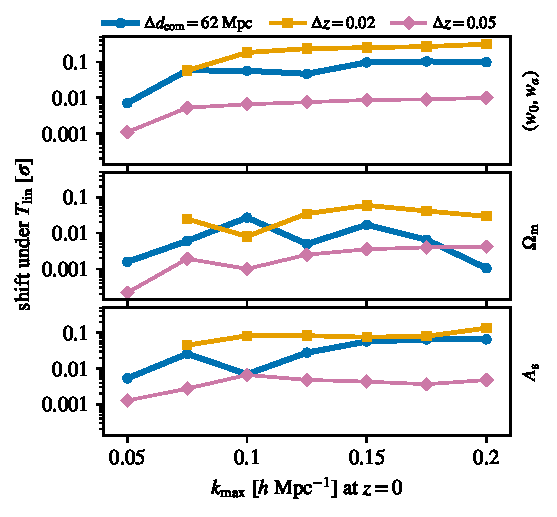
\includegraphics[width=0.72\linewidth]{plots/tlin_shift_kmax/tlin_shift_kmax.pdf}
  \caption{The shift of today's model V0 when the true dispersions
    follow the linear flow's own redshift dependence (the truth
    $T_{\rm lin}$), against the scale cut.  Top to bottom:
    $(w_0, w_a)$ in units of its error ellipse,
    $\sqrt{\Delta p^{\mathsf T} C^{-1} \Delta p}$ with $C$ the pair's
    $2 \times 2$ marginalized covariance, then $\Omega_m$ and $A_s$
    in units of their own $\sigma$.  The $\Delta z = 0.2$ layout is
    not drawn: its shifts stay below $10^{-3}\,\sigma$.  On
    $\Delta z = 0.02$ no band survives the $\kmax = 0.05\hMpc$ cut,
    so its curve starts at $0.075$.  $\kmax$ quoted at $z = 0$; each
    bin is cut at $\kmax/D(\bar{z}_i)$.}
  \label{fig:tlinshift}
\end{figure}

\paragraph{The numbers.}
On $\Delta z = 0.02$ the $(w_0, w_a)$ fit moves by $0.06$ of its
error ellipse at $\kmax = 0.075$, $0.18$ at $0.1$ and $0.32$ at
$0.2$; $A_s$ moves by $0.04$--$0.14\,\sigma$ and $\Omega_m$ by
$0.01$--$0.06\,\sigma$.  On \dcom{} the ellipse shift is $0.007$ at
$0.05$, $0.05$--$0.06$ at $0.075$--$0.125$ and about $0.10$ at
$0.15$--$0.2$, with $A_s$ up to $0.07\,\sigma$ and $\Omega_m$ up to
$0.03\,\sigma$.  On $\Delta z = 0.05$ the ellipse shift stays at
$0.001$--$0.010$ and the single parameters below $0.007\,\sigma$; on
$\Delta z = 0.2$ everything is below $2 \times 10^{-4}$.

\paragraph{Why the thin layouts are the sensitive ones.}
The ordering of the layouts is the edge-fraction argument of the
cross-correlation note: a Gaussian blur of width $\sigma_z$ moves a
fraction of about $\sigma_z/(\sqrt{2\pi}\,w_{\rm bin})$ of a bin's
galaxies across each edge, with $w_{\rm bin}$ the bin's width in
redshift, so the thinner the bin, the larger the share of its
galaxies the blur relocates -- and the more strongly its spectra
respond to its $\sv$.  The widths, worked at the fiducial cosmology:
a $\Delta z$ bin is $c\,\Delta z/H(z)$ deep, and with
$H(0.95) = 115\kms/{\rm Mpc}$ a $\Delta z = 0.02$ bin is
$299792 \times 0.02/115 \approx 52$~Mpc deep at $z = 0.95$, falling
to $37$~Mpc at $z = 1.55$ ($H = 160\kms/{\rm Mpc}$): thinner than the
fixed $62$~Mpc bins exactly where the ELG groups put most of their
bins, which is why $\Delta z = 0.02$ overtakes \dcom{} in
Figure~\ref{fig:tlinshift}.  The same arithmetic makes a
$\Delta z = 0.05$ bin $90$--$130$~Mpc deep there, twice the $62$~Mpc
width, and a $\Delta z = 0.2$ bin several hundred Mpc deep.  The
shift also grows with the cut, because raising $\kmax$ admits more
bands, and the bands it adds are the small-scale ones where the
blur's suppression -- the Fingers-of-God damping of
Section~\ref{sec:what} -- is strongest, so the data's sensitivity to
each bin's $\sv$ grows with it.

\subsection{Error bars under the random truths}
\label{sec:res-eta}

\paragraph{The truth and the baseline.}
The ensemble truth $T_{\rm lin} + {\rm B}$ adds to the fixed
$T_{\rm lin}$ shape random draws of the halo-part slope (at the
baseline width $1.0$) and of residual B, as in
Figure~\ref{fig:draws}.  As in the project's other notes, the
ensemble also draws the linear-bias truths of the paper prior and the
data noise, so the test scores the whole fit, not the dispersions in
isolation; with no $\sv$ truth at all it returns
$\eta = 1.0000$ on every layout and cut -- the honest baseline every
departure below is measured from.  Figure~\ref{fig:sigveta} shows
$\eta$ for V0 and for V1 at the baseline slope width.

\begin{figure}[tbp]
  \centering
  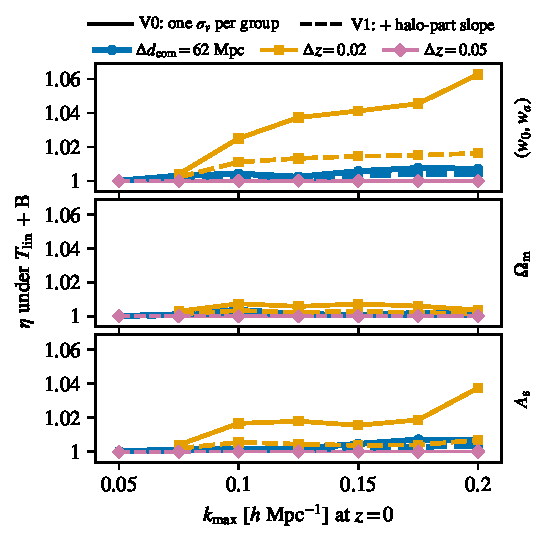
\includegraphics[width=0.72\linewidth]{plots/sigv_eta_kmax/sigv_eta_kmax.pdf}
  \caption{How well each fit's quoted error bar covers where the fit
    actually lands, measured by $\eta$ ($\eta = \chidof$ with
    $\chi^2 = \Delta p^{\mathsf T} C_p^{-1} \Delta p$,
    Section~\ref{sec:study}; $\eta = 1$ means honest error bars),
    under the truth $T_{\rm lin} + {\rm B}$, against the scale cut.
    Today's model V0 (solid) and the slope variant V1 at the baseline
    width (dashed); top to bottom: $(w_0, w_a)$, $\Omega_m$, $A_s$.
    The $\Delta z = 0.2$ layout is not drawn: its $\eta$ differs from
    one by less than $10^{-5}$.  The other slope widths and residual
    variants are quoted in the text.  $\kmax$ quoted at $z = 0$; each
    bin is cut at $\kmax/D(\bar{z}_i)$.}
  \label{fig:sigveta}
\end{figure}

\paragraph{The numbers.}
For V0 on $\Delta z = 0.02$, $\eta$ of $(w_0, w_a)$ is $1.004$ at
$\kmax = 0.075$, $1.025$ at $0.1$, $1.037$--$1.046$ at
$0.125$--$0.175$ and $1.063$ at $0.2$; $A_s$ reaches $1.037$ and
$\Omega_m$ $1.007$.  On \dcom{} V0 stays at or below $1.0076$ for
$(w_0, w_a)$, $1.007$ for $A_s$ and $1.004$ for $\Omega_m$; on
$\Delta z = 0.05$ at or below $1.0002$.  The slope alone repairs most
of this: V1 at the baseline width keeps $(w_0, w_a)$ at
$1.002$--$1.016$ on $\Delta z = 0.02$ ($A_s$ at most $1.007$,
$\Omega_m$ at most $1.003$) and at most $1.004$ on \dcom.  At the
hardest point -- $\kmax = 0.2$, $\Delta z = 0.02$, $(w_0, w_a)$ --
the other variants: V1 at width $0.5$ gives $1.043$, at width $2.0$
$0.998$ (error bars slightly wider than the actual scatter); V2
(slope $+$ residual A) $1.016$; V3 (slope $+$ residual B) $1.014$,
unchanged by the white term; V4 $1.0001$.  Under the random draws
alone, with no $T_{\rm lin}$, the same point gives V0 $1.039$, V1
$1.005$ and V3 $1.004$; under $T_{\rm lin}$ alone V0 gives $1.025$.
Both loads matter for today's model.  The quantity that adds over
independent truths is $\eta^2 - 1$ (the truths' contributions to
$\langle\chi^2\rangle$ add), and for V0 the random draws contribute
$1.039^2 - 1 \approx 0.080$ and $T_{\rm lin}$
$1.025^2 - 1 \approx 0.050$, which together give
$\sqrt{1.130} \approx 1.063$.  The two loads respond differently to
the slope: V1 removes almost all of the random load, while most of
the $T_{\rm lin}$ shift survives it.  Isolating
that shape, the $T_{\rm lin}$ shift of $(w_0, w_a)$ at this point
falls along the family as $0.32$ (V0), $0.28$ (V1, width $0.5$),
$0.21$ (width $1.0$), $0.12$ (width $2.0$), $0.21$ (V2 and V3) and
$0.011$ (V4).

\paragraph{Why the slope absorbs only part of $T_{\rm lin}$.}
In halo-part units the $T_{\rm lin}$ tilt is large, because the halo
share $w$ is small.  Worked on ELG2 with
Table~\ref{tab:decomposition} and the group ranges of
Section~\ref{sec:fiducial}: ELG2 has $w = 0.17$ and $25$ bins
spanning $\Delta z \approx 0.5$, and $T_{\rm lin}$ moves its
dispersions by up to $3.4\%$ of $\svg$ at the group ends (the $-9$ to
$+10\kms$ of Section~\ref{sec:study}).  Dividing by $w$, that is a
$3.4/0.17 \approx 20\%$ tilt of $\shod$ across half the group ($0.25$
in $z$): a slope of about $0.8$ per unit $z$, close to one sigma of
the baseline slope prior.  A Gaussian prior pulls the fitted slope
back toward its center at zero, so V1 absorbs only part of the tilt;
the $2.0$ width absorbs more, and V4, with no shape prior at all,
absorbs essentially all of it.  The residuals cannot absorb a tilt
either: their directions are projected so that they carry neither a
level nor a slope component (Section~\ref{sec:model}), which is why
V2 and V3 sit on top of V1 under $T_{\rm lin}$.

\subsection{The cost of the freedom}
\label{sec:res-cost}

\paragraph{The numbers.}
Figure~\ref{fig:sigvfom} gives the price, as the loss of each FoM
against V0.  V1 at the baseline width costs, on $\Delta z = 0.02$,
$0.3\%$ of FoM$(w_0, w_a)$ at $\kmax = 0.075$, $1.6\%$ at $0.1$,
$2.3$--$2.6\%$ at $0.125$--$0.175$ and $3.4\%$ at $0.2$ ($2.6\%$ of
FoM$(\Omega_m, 10^9 A_s)$ there); on \dcom{} at most $0.5\%$, on
$\Delta z = 0.05$ at most $0.011\%$ and on $\Delta z = 0.2$ below
$3 \times 10^{-5}$ percent.  The other variants at $\kmax = 0.2$,
FoM$(w_0, w_a)$: on $\Delta z = 0.02$, V1 at width $0.5$ costs
$1.2\%$, at width $2.0$ $6.2\%$, V2 $3.4\%$, V3 $3.6\%$, V3 with the
white term $3.6\%$; on \dcom{}, V1 at width $2.0$ costs $1.3\%$ and
V3 $0.5\%$; on $\Delta z = 0.05$ everything stays at or below
$0.04\%$.  V4, the bound, costs at $\kmax = 0.2$: $6.1$, $11.2$,
$5.0$ and $0.4\%$ of FoM$(w_0, w_a)$ and $6.4$, $8.5$, $7.7$ and
$2.9\%$ of FoM$(\Omega_m, 10^9 A_s)$ on \dcom{} / $\Delta z = 0.02$
/ $0.05$ / $0.2$.  At the low cuts the bound is expensive: $59\%$
(\dcom{} at $0.05$), $48\%$ ($\Delta z = 0.02$ at $0.075$) and
$30\%$ ($\Delta z = 0.05$ at $0.05$) of FoM$(w_0, w_a)$, and up to
$72\%$ of FoM$(\Omega_m, 10^9 A_s)$ (\dcom{} at $0.05$).

\begin{figure}[tbp]
  \centering
  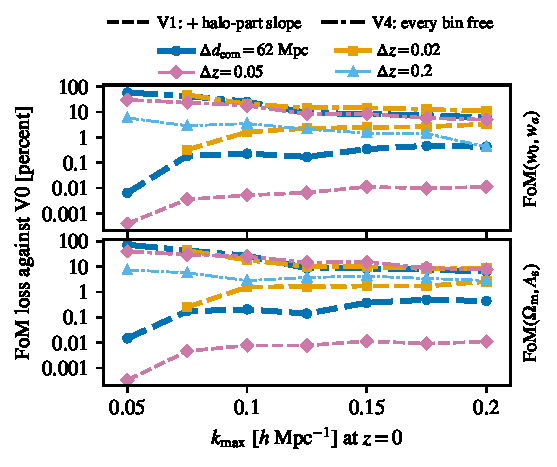
\includegraphics[width=0.72\linewidth]{plots/sigv_fom_loss_kmax/sigv_fom_loss_kmax.pdf}
  \caption{The cost of the per-bin freedom: the loss of
    FoM$(w_0, w_a)$ (top) and FoM$(\Omega_m, 10^9 A_s)$ (bottom)
    against today's model V0, in percent, for the slope variant V1
    at the baseline width (dashed) and for the bound V4, every bin's
    dispersion free (dash--dotted).  V1 on $\Delta z = 0.2$ is not
    drawn: its loss stays below $10^{-4}$ percent.  The other slope
    widths and the residual variants are quoted in the text.
    $\kmax$ quoted at $z = 0$; each bin is cut at
    $\kmax/D(\bar{z}_i)$.}
  \label{fig:sigvfom}
\end{figure}

\paragraph{Why the residuals are nearly free, and the bound is not.}
V2 and V3 cost at most $0.2$ percentage points more than V1: their
prior is projected
(no level, no slope) and tight once expressed in $\sv$ units -- a
residual of $20\%$ of $\shod$ reaches $\sv$ multiplied by the halo
share, and $w \times 20\%$ is a few percent
(Table~\ref{tab:priors}) -- so the wiggle directions they open are
directions the prior immediately closes.  V4 is expensive at low
cuts for a different reason -- the likely one, not tested separately
here: with few bands kept per bin, a small
change of a bin's $\sv$ and a small change of its linear bias
$b_{1,i}$ move those few bands nearly proportionally, so the per-bin
dispersion and the per-bin bias are nearly degenerate, and freeing
both per bin lets that degeneracy eat the FoM.  As the cut rises the
bands separate the two effects and the cost of the bound falls to
the $5$--$11\%$ above.

\subsection{Numerical checks}
\label{sec:checks}

\paragraph{The whitened norm.}
The checks below measure changes of the data vector in the whitened
norm $\|x\| = \sqrt{x^{\mathsf T} G x}$ with
$G = B^{\mathsf T} C^{-1} B$.  Here the columns of $B$ are the
derivative columns of the base (each the change of the whole data
vector per unit change of one parameter), $x$ holds the coefficients
of a change in that base, so $Bx$ is the change of the data vector
itself, and $C$ is the data covariance of the bands the shipped mask
keeps: $x^{\mathsf T} G x = (Bx)^{\mathsf T} C^{-1} (Bx)$ is the
$\chi^2$ of that change.  ``Whitened'' means the change is
expressed in units of the data's own error bars, every band weighted
by how well it is measured: a norm of $1$ is a change of the data
the size of its one-sigma noise.

\paragraph{Four checks.}
\begin{itemize}
  \item \textbf{Group sum.}  The sum of a group's per-bin $\sv$
    columns reproduces the group's own $\sv$ column of the paper's
    derivative base -- an independent calculation -- to
    $0.1$--$0.5\%$ in the whitened norm: at worst $0.54\%$
    ($\Delta z = 0.05$), $0.11\%$ ($\Delta z = 0.02$), $0.16\%$
    (\dcom) and $0.15\%$ ($\Delta z = 0.2$).
  \item \textbf{Reproduction of the notebook.}  V0 of the study
    reproduces the Fisher notebook's FoM and its $\eta$ to $10^{-9}$
    (the study reuses the notebook's own fit cells).
  \item \textbf{Reset.}  The model evaluated at the fiducial before
    and after all the steps agrees exactly (difference $0$).
  \item \textbf{Step test.}  Per-bin columns from relative steps
    $0.01$ and $0.04$ differ from the step-$0.02$ columns by
    $3.5$--$5\%$ ($\Delta z = 0.2$ and \dcom) and $8$--$10\%$
    ($\Delta z = 0.02$ and $0.05$) in the whitened norm, column by
    column.  The whole study was refitted with step $0.01$ and with
    step $0.04$ as the main step (the fits only; the caches hold all
    three steps): every number of
    Figures~\ref{fig:tlinshift}--\ref{fig:sigvfom} except V4 is
    unchanged to the third digit -- on $\Delta z = 0.02$ at
    $\kmax = 0.2$ the $T_{\rm lin}$ shift of $(w_0, w_a)$ is
    $0.3152$ / $0.3152$ / $0.3151$ for steps $0.01$ / $0.02$ /
    $0.04$, $\eta$ of V0 under $T_{\rm lin} + {\rm B}$ is $1.0627$
    at all three, and the V1 loss is $3.349$ / $3.347$ / $3.346\%$.
    V4's losses move by at most $0.2$ percentage points, except
    $\Delta z = 0.05$ at $\kmax = 0.05$ with step $0.04$
    ($30.0$ / $30.0$ / $36.3\%$), where few bands are kept.
\end{itemize}
Two of these numbers deserve a plain-words reading.  First, how can
a $10\%$ difference between derivative columns leave every shift and
FoM unchanged to the third digit?  Because the difference lives in
the per-bin directions the data barely constrain: those directions'
errors are set by the priors, not by the columns' small details, so
the columns can wobble there without moving any score.  Second, the
group-sum check is best at step $0.02$ ($0.1$--$0.5\%$, against
$1$--$4\%$ at $0.01$ and $0.04$) -- and $0.02$ is the step of the
paper base's own group columns, exactly as expected when the two
sides of the comparison share the same stencil.

\subsection{What to remember, and an option}
\label{sec:remember}

\begin{itemize}
  \item The linear flow's decline across each group is a
    deterministic mismatch of today's flat-$\sv$ model, fixed in
    sign and size by the fiducial cosmology: it moves the
    $(w_0, w_a)$ fit by up to a third of its error ellipse on the
    thinnest layout at $\kmax = 0.2\hMpc$.
  \item One free halo-part slope per group restores most of the
    error bars' honesty ($\eta$ from $1.063$ to $1.016$) at a cost
    of at most a few percent of either FoM, but absorbs only a third
    of the $T_{\rm lin}$ shift: the slope $T_{\rm lin}$ implies is
    about one sigma of the baseline prior, so the prior shrinks the
    fitted slope partway and a shift of a fifth of the ellipse
    remains.
  \item The projected residuals buy almost nothing and cost almost
    nothing: they carry neither a level nor a slope, and in $\sv$
    units their priors are a few percent.
  \item Every per-bin $\sv$ free is the expensive bound, because at
    low cuts a bin's dispersion and its linear bias are nearly
    degenerate in the few kept bands.
  \item Thin bins are the sensitive ones: the blur relocates a share
    $\sigma_z/(\sqrt{2\pi}\,w_{\rm bin})$ of a bin's galaxies, and
    the $\Delta z = 0.02$ bins are $37$--$52$~Mpc deep at
    $z \gtrsim 1$, so that layout responds most and
    $\Delta z = 0.2$ barely at all.
\end{itemize}

\paragraph{An option: carry the linear part in the fiducial.}
The $T_{\rm lin}$ shape is not a nuisance to marginalize: it is
fixed by the fiducial cosmology (Section~\ref{sec:linear}).  A model
whose fiducial carries it --
$\sv^2{}_{,i} = \slin^2(\bar{z}_i) + \shod^2{}_{,g}$, with one free
level per group exactly as today -- would remove the $T_{\rm lin}$
shift with no new parameter, hence at no FoM cost to first order,
and would leave the slope prior to cover the halo part's own
evolution.  It changes the fiducial dispersions by up to $10\kms$,
so the paper's derivative bases would be out of date and the
expensive derivatives would have to be recomputed at the new
fiducial.  Whether to do that is the project lead's decision (the
appendix lists it).  A cheaper intermediate needs no new
derivatives: center V1's slope prior on the slope $T_{\rm lin}$
implies instead of on zero.

\appendix

\section{Open issues}
\label{app:open}

\paragraph{Runs.}
The derivative columns, the step test, the group-sum check, the
accuracy test and the FoM variants are done
(Section~\ref{sec:results}).  Still open, and optional: the same
per-bin columns on the largest-pair-list bases.  The refits with
$w \pm 0.05$ are closed without new runs: $w$ enters only as the
factor multiplying the halo-part widths (Eq.~\eqref{eq:response}),
so a change of $w$ by $0.05$ -- $17$--$35\%$ of $w$ -- rescales
every halo-part prior by that factor, well inside the
$0.5$--$2.0$ slope-width bracket the study already computed.

\paragraph{Decisions for the project lead.}
\begin{itemize}
  \item \textbf{The linear-part template.}  Whether to build the
    linear flow's redshift dependence into the fiducial
    (Section~\ref{sec:remember}): it removes the $T_{\rm lin}$
    shift with no new parameter, and it makes the paper's
    derivative bases out of date, so the expensive derivatives must
    be recomputed at the new fiducial.  The cheap intermediate --
    centering the slope prior on the slope $T_{\rm lin}$ implies --
    needs no new derivatives.
  \item \textbf{The source forecast's per-bin $\sv(\bar{z})$ figure}
    is not available now.  The priors of Table~\ref{tab:priors}
    stand on the literature and the halo model; when the figure turns
    up, a $\chi^2$ of its points against a flat line per group bounds
    the real bin-to-bin scatter, and $\sigma$, $L$ and the slope
    widths are refitted in minutes with no new derivatives.
  \item \textbf{Robustness study or fiducial-model candidate?}
    Whether a per-bin variant that passes the accuracy test is a
    check on today's model or a candidate to replace it decides
    whether the summary note changes.
  \item \textbf{Confirm the halo-part priors} of
    Table~\ref{tab:priors} (slope widths, A, B, BGS factors) and
    whether the white term is included.
  \item \textbf{BGS flux-limited} is settled project-wide (the bias
    drift already comes from the flux limit), fixing its slope width
    at $2.0$; reopen only with that decision.
\end{itemize}

\paragraph{Open physics items.}
\begin{itemize}
  \item \textbf{The ELG halo part is model dependent at the
    factor-two level} (Section~\ref{sec:sum}): the subtraction gives
    $114$--$119\kms$ against $76$--$145\kms$ from the two published
    occupations.  Fractional priors on $\shod$ absorb this; an
    absolute prior would not.
  \item \textbf{The blur's Gaussian shape} against the mixture's
    heavier tails (Section~\ref{sec:caveats}) is an open robustness
    check on the profile, separate from the per-bin amplitude freedom
    studied here.
  \item \textbf{The Kaiser boundary}: damping with the full one-point
    $\sv$ versus the halo part alone
    (Section~\ref{sec:caveats}) is a modeling convention the project
    inherits from the source forecast; the wide paper priors cover
    it, and no result of this study depends on settling it.
  \item \textbf{Mass-definition conversions} (CompaSO to $M_{200c}$,
    Section~\ref{sec:virial}) shift $\shalo$ by $1$--$3\%$ and are
    absorbed into the priors; a precision reanalysis of the halo
    model would apply them explicitly.
  \item \textbf{The halo-motion part} is linear theory with a
    several-percent uncertainty of either sign
    (Section~\ref{sec:linear}); it reaches the study only through
    $w$, and the $w \pm 0.05$ rescaling argument above bounds its
    effect inside the computed slope-width bracket.
\end{itemize}

\begin{thebibliography}{99}

\bibitem{Jackson1972}
J.~C. Jackson,
``A critique of Rees's theory of primordial gravitational radiation'',
MNRAS 156 (1972) 1P.

\bibitem{Kaiser1987}
N. Kaiser,
``Clustering in real space and in redshift space'',
MNRAS 227 (1987) 1.

\bibitem{Evrard2008}
A.~E. Evrard et al.,
``Virial scaling of massive dark matter halos: why clusters prefer a
high normalization cosmology'',
ApJ 672 (2008) 122, arXiv:astro-ph/0702241.

\bibitem{Zheng2007}
Z. Zheng, A.~L. Coil and I. Zehavi,
``Galaxy evolution from halo occupation distribution modeling of DEEP2
and SDSS galaxy clustering'',
ApJ 667 (2007) 760, arXiv:astro-ph/0703457.

\bibitem{Yuan2022}
S. Yuan, L.~H. Garrison, B. Hadzhiyska, S. Bose and D.~J. Eisenstein,
``AbacusHOD: a highly efficient extended multi-tracer HOD framework
and its application to BOSS and eBOSS data'',
MNRAS 510 (2022) 3301, arXiv:2110.11412.

\bibitem{Yuan2023}
S. Yuan et al.,
``The DESI One-Percent Survey: exploring the halo occupation
distribution of luminous red galaxies and quasi-stellar objects with
AbacusSummit'',
MNRAS 530 (2024) 947, arXiv:2306.06314.

\bibitem{Rocher2023}
A. Rocher et al.,
``The DESI One-Percent Survey: exploring the halo occupation
distribution of emission line galaxies with AbacusSummit
simulations'',
JCAP 10 (2023) 016, arXiv:2306.06319.

\bibitem{Hadzhiyska2022}
B. Hadzhiyska, D. Eisenstein, S. Bose, L.~H. Garrison and
N. Maksimova,
``CompaSO: a new halo finder for competitive assignment to spherical
overdensities'',
MNRAS 509 (2022) 501, arXiv:2110.11408.

\bibitem{BryanNorman1998}
G.~L. Bryan and M.~L. Norman,
``Statistical properties of X-ray clusters: analytic and numerical
comparisons'',
ApJ 495 (1998) 80, arXiv:astro-ph/9710107.

\bibitem{Favole2025}
G. Favole, F.-S. Kitaura, B. Hadzhiyska, D.~J. Eisenstein,
L.~H. Garrison and S. Bose,
``ELG$\times$LRG distribution through dark matter halo dynamics'',
ApJ 1002 (2026), arXiv:2512.04362.

\bibitem{ShethTormen1999}
R.~K. Sheth and G. Tormen,
``Large scale bias and the peak background split'',
MNRAS 308 (1999) 119, arXiv:astro-ph/9901122.

\bibitem{White2001}
M. White,
``The redshift-space power spectrum in the halo model'',
MNRAS 321 (2001) 1, arXiv:astro-ph/0005085.

\bibitem{Seljak2001}
U. Seljak,
``Redshift-space bias and $\beta$ from the halo model'',
MNRAS 325 (2001) 1359, arXiv:astro-ph/0009016.

\bibitem{Maus2024}
M.~Maus, S.~Chen, M.~White et al.,
``An analysis of parameter compression and full-modeling techniques
with Velocileptors for DESI 2024 and beyond'',
2024, arXiv:2404.07312.

\bibitem{BBKS1986}
J.~M. Bardeen, J.~R. Bond, N. Kaiser and A.~S. Szalay,
``The statistics of peaks of Gaussian random fields'',
ApJ 304 (1986) 15.

\bibitem{ShethDiaferio2001}
R.~K. Sheth and A. Diaferio,
``Peculiar velocities of galaxies and clusters'',
MNRAS 322 (2001) 901, arXiv:astro-ph/0009166.

\bibitem{Marzke1995}
R.~O. Marzke, M.~J. Geller, L.~N. da Costa and J.~P. Huchra,
``Pairwise velocities of galaxies in the CfA and SSRS2 redshift
surveys'',
AJ 110 (1995) 477, arXiv:astro-ph/9504070.

\bibitem{Loveday2018}
J. Loveday et al.,
``Galaxy and Mass Assembly (GAMA): small-scale anisotropic galaxy
clustering and the pairwise velocity dispersion of galaxies'',
MNRAS 474 (2018) 3435, arXiv:1711.05636.

\bibitem{Tinker2007}
J.~L. Tinker, P. Norberg, D.~H. Weinberg and M.~S. Warren,
``On the luminosity dependence of the galaxy pairwise velocity
dispersion'',
ApJ 659 (2007) 877, arXiv:astro-ph/0603543.

\bibitem{Beutler2017}
F. Beutler et al.,
``The clustering of galaxies in the completed SDSS-III Baryon
Oscillation Spectroscopic Survey: anisotropic galaxy clustering in
Fourier space'',
MNRAS 466 (2017) 2242, arXiv:1607.03150.

\bibitem{Pezzotta2017}
A. Pezzotta et al.,
``The VIMOS Public Extragalactic Redshift Survey (VIPERS): the growth
of structure at $0.5 < z < 1.2$ from redshift-space distortions in
the clustering of the PDR-2 final sample'',
A\&A 604 (2017) A33, arXiv:1612.05645.

\bibitem{SalazarAlbornoz2017}
S. Salazar-Albornoz et al.,
``The clustering of galaxies in the completed SDSS-III Baryon
Oscillation Spectroscopic Survey: angular clustering tomography and
its cosmological implications'',
MNRAS 468 (2017) 2938, arXiv:1607.03144.

\bibitem{GrasshornGebhardt2020}
H.~S. Grasshorn Gebhardt and D. Jeong,
``Nonlinear redshift-space distortions in the harmonic-space galaxy
power spectrum'',
Phys. Rev. D 102 (2020) 083521, arXiv:2008.08706.

\bibitem{Jalilvand2020}
M. Jalilvand, B. Ghosh, E. Majerotto, B. Bose, R. Durrer and M. Kunz,
``Nonlinear contributions to angular power spectra'',
Phys. Rev. D 101 (2020) 043530, arXiv:1907.13109.

\end{thebibliography}

\end{document}
